\documentclass[12pt]{article}
\usepackage{amsmath, amssymb, amsthm}    
\usepackage{parskip}  
\usepackage{enumitem}  
\usepackage{geometry}    
\usepackage{titling}     
\usepackage{color}       
\usepackage{hyperref}   
\usepackage{tipa}
\usepackage{graphicx}     
\usepackage{mathrsfs}
\usepackage{tikz}
\usepackage{tkz-euclide}
\usepackage[toc,page]{appendix} 
\usepackage{listings}
\allowdisplaybreaks %% TODO: IS IT THAT BAD TO SPLIT EQUATION STRINGS BETWEEN PAGES?

%\usepackage{showkeys} %so you can see your labels; take out when working with final draft
\usepackage[v2]{xy}
\usepackage{amscd}  

%\linespread{2}
\setlength{\parindent}{3em}   
\setlength{\parskip}{1em}   
%\setlength{\droptitle}{-5em}

% Sets
\newcommand{\N}{\mathbb{N}}
\newcommand{\Z}{\mathbb{Z}}
\newcommand{\R}{\mathbb{R}}
\newcommand{\C}{\mathbb{C}}
\newcommand{\fc}{F^{\C}}

% Matrices
\newcommand{\lftmat}[4]{\begin{bmatrix} {#1} & {#2} \\ {#3} & {#4} \end{bmatrix}}
\newcommand{\stanlftmat}{\lftmat{a}{b}{c}{d}}
\newcommand{\pointmat}[2]{\lftmat{{#2}}{{#1}}{-1}{-{#2}}}
\newcommand{\stanpointmat}{\pointmat{x}{y}}
\newcommand{\linenoendmat}[2]{\begin{bmatrix} -{#2} & -{#1} \\ 1 & {#2} \end{bmatrix}}
\newcommand{\stanlinenoendmat}{\linenoendmat{l_1}{l_2}}
\newcommand{\lineendmat}[2]{\begin{bmatrix} -1 & -{#1} \\ 0 & 1 \end{bmatrix}}
\newcommand{\stanlineendmat}{\lineendmat{l_1}{l_2}}

% Spacing
\newcommand{\spceq}{\hspace{2mm} = \hspace{2mm}}
\newcommand{\ttspc}{\hspace{1mm}}
\newcommand{\ttc}{, \hspace{1mm}}

% Miscellaneous
\newcommand{\poincare}{Poincar\'{e} }
\newcommand{\Tr}{\text{Tr}}
\newcommand{\Range}{\text{Range}}
\newcommand{\Ker}{\text{Ker}}
\newcommand{\inv}{^{-1}}
\newcommand{\Log}{\text{Log}}
\newcommand{\specialend}{(\infty^2\ttc\infty)}

% Colors for listings
\definecolor{orange}{rgb}{1,0.5,0}
\definecolor{purple}{rgb}{.5,0,0.5}
\definecolor{dgreen}{rgb}{.1, .7, .2}
\definecolor{codegreen}{rgb}{0,0.6,0}
\definecolor{codegray}{rgb}{0.5,0.5,0.5}
\definecolor{codepurple}{rgb}{0.58,0,0.82}
\definecolor{backcolour}{rgb}{0.95,0.95,0.92}
 
% Listings style
\lstdefinestyle{mystyle}{
    backgroundcolor=\color{backcolour},   
    commentstyle=\color{codegreen},
    keywordstyle=\color{magenta},
    numberstyle=\tiny\color{codegray},
    stringstyle=\color{codepurple},
    basicstyle=\footnotesize,
    breakatwhitespace=false,         
    breaklines=true,                 
    captionpos=b,                    
    keepspaces=true,                 
    numbers=left,                    
    numbersep=5pt,                  
    showspaces=false,                
    showstringspaces=false,
    showtabs=false,                  
    tabsize=2
}
\lstset{style=mystyle}

% Theorem counters
\theoremstyle{plain}
\newtheorem{theorem}{Theorem}[section]
\newtheorem{definition}{Definition}[section]
\newtheorem{corollary}[theorem]{Corollary}
\newtheorem{lemma}[theorem]{Lemma}
\newtheorem{proposition}[theorem]{Proposition}

% Spacing for theorems
\makeatletter
\def\thm@space@setup{%
  \thm@preskip=\parskip \thm@postskip=0pt
}
\makeatother

% Problem environments
\theoremstyle{definition}
\newtheorem{problem}[theorem]{Problem}
\newtheorem{example}[definition]{Example}


\newcommand{\todo}[1]{\color{magenta} \text{{#1}} \color{black}}


\title{The Hyperbolic Geometry of Linear Fractional Transformations in the \poincare Disk}
\author{Anna Blinderman, Logan Goldberg}
\date{}

\begin{document}
\maketitle

\begin{abstract}
In his paper \textit{The Hilbert Model of Hyperbolic Geometry}, Heinrich Guggenheimer classifies linear fractional transformations with coefficients in a real, ordered field $F$ as point reflections and line reflections. In this paper we first introduce a clear notation for such transformations and motivate the algebra behind Guggenheimer's classifications wherever possible. We then illustrate the effects of such linear fractional transformations with coefficients in $F = \R$ using the \poincare disk model for hyperbolic geometry. Motivated by Guggenheimer's claim that this geometry can be developed similarly for transformations with coefficients in $\fc$ (the complexified\footnote{See Appendix \ref{appendixB}.} version of $F$), we attempt to do so for $\R^{\C}$ (i.e. $\C$). Finally, we point out issues with Guggenheimer's development of this geometry in $\R$ and raise questions about his claim that these conventions can be applied in complexified fields, particularly $\C$. \todo{[AB][LG] do we have to cite the paper somewhere in there?}
\end{abstract}



%%%%%%%%%%%%%%%%%%%%%%%%%%%%%%%%%%%%%%%%%%%%%%%%%%%%%%%%
\section{Introduction}

\hspace{10mm} For centuries, mathematicians tried tirelessly to prove that Euclid's fifth postulate -- an equivalent formulation of the parallel postulate -- followed from the first four. It was not until the 19$^{\text{th}}$ century that Carl Friedrich Gauss and J\'{a}nos Bolyai showed that the the fifth postulate was independent from the others. This shocking result opened doors to the exploration of non-Euclidean geometric models, particularly those of hyperbolic geometry \cite{hartshorne}.

To understand hyperbolic geometry we must first consider the five postulates that axiomatize Euclidean geometry. The first four are as follows\footnote{[\cite{hartshorne}, p.~481]}:
\begin{enumerate}[leftmargin = 4em, itemsep=-.8em]
	\item A straight line segment can be drawn joining any two points.
	\item Any straight line segment can be extended indefinitely in a straight line.
	\item Given any straight line segment, a circle can be drawn having the segment as radius and one endpoint as center.
	\item All right angles are congruent.
\end{enumerate}
These all hold in hyperbolic geometry. However, the fifth postulate
\begin{enumerate}[leftmargin = 4em, itemsep=-1em]
	\setcounter{enumi}{4}
	\item Given a line and a point not on that line, at most one line parallel to the given line can be drawn through that line.
\end{enumerate}
is replaced with a stronger negation: ``Through an exterior point to a straight line we can construct an infinite number of parallels to that straight line.'' \cite{euclids_fifth}. We will mainly be working with infinite fields, so it is more helpful to us to appeal to this stronger negation than its weaker negation ``Through an exterior point to a straight line, we can construct at least two lines parallel to it.'' 

As demonstrated below, line $m$ is the unique line through $P$ parallel to $l$ in Euclidean geometry while lines $n_1$ and $n_2$ through $P$ are parallel to $l$ in hyperbolic geometry.

\begin{center}
\begin{tabular}{cc}
	\begin{tikzpicture}
		\draw[fill=black] (-1,1) circle (0.05) node[right] {$P$};
		\draw (-2,-2) -- (2,2) node[right] {$l$};
		\draw (-2,0) -- (0,2) node[right] {$m$};
	% Playfair's axiom
	\end{tikzpicture} 
	& 	
	\begin{tikzpicture}
		\draw[fill=black] (-1,1) circle (0.05) node[right] {$P$};
		\draw (-2,-2) -- (2,2) node[right] {$l$};
		\draw (-1.5,.835) arc (-80:-40:2cm) node[right] {$n_1$};
		\draw (-1.43,.5) arc (-50:-10:2cm) node[left] {$n_2$};
	% Hyperbolic axiom
	\end{tikzpicture}   \\
Fifth postulate in Euclidean geometry & Fifth postulate in hyperbolic geometry \\
& \\
\end{tabular}
\end{center}
In the Euclidean model, $m$ is the unique line through $P$ and parallel to $l$. On the other hand, in the hyperbolic model we have that $n_1$ and $n_2$ are distinct lines passing through $P$ and parallel to $l$. 

Henri \poincare put forth two models for visualizing hyperbolic geometry: the \poincare half-plane and the \poincare disk. We focus here on the disk model. Let $\Gamma$ be any circle in the Cartesian plane and call its center $O$. The set of points in this model is the interior of $\Gamma$ \cite{hartshorne}. A line in this model is the collection of all model points that lie on a circle that is orthogonal to $\Gamma$ or that lie on a Euclidean line through $O$. Consider the following figure: 

\begin{center}
	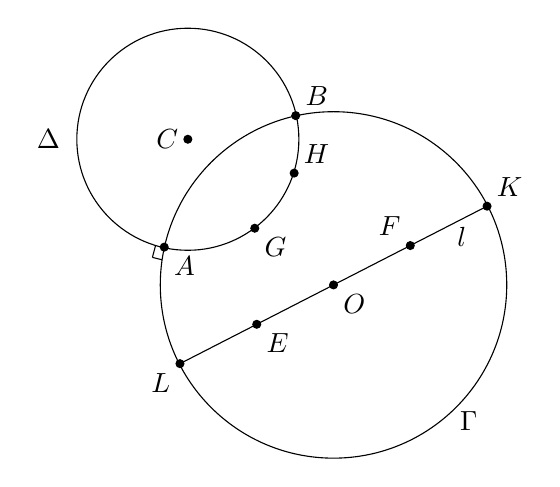
\begin{tikzpicture}
	\draw (0,0) circle (2.2cm) node[below right=2.1cm] {$\Gamma$};
	\draw (-1.85,1.85) circle (1.41cm) node[left=1.5cm] {$\Delta$};
	\draw[fill=black] (0,0) circle (0.05) node[below right] {$O$};
	\draw[fill=black] (-1.85,1.85) circle (0.05) node[left] {$C$};
	\draw[fill=black] (-2.15,.48) circle (0.05) node[below right] {$A$};
	\draw[fill=black] (-.48,2.15) circle (0.05) node[above right] {$B$};
	\draw[fill=black] (-1.95,-1) circle (0.05) node[below left] {$L$};
	\draw[fill=black] (1.95,1) circle (0.05) node[above right] {$K$};
	\draw[fill=black] (-0.975,-.5) circle (0.05) node[below right] {$E$};
	\draw[fill=black] (0.975,.5) circle (0.05) node[above left] {$F$};
	\draw[fill=black] (-1,.72) circle (0.05) node[below right] {$G$};
	\draw[fill=black] (-.5,1.42) circle (0.05) node[above right] {$H$};
	(-2.15,.48)
	\draw (-1.95, -1) -- (1.95, 1) node[below left=.2cm] {$l$};
	\draw (-2.3,.35)  -- (-2.26,.5);
	\draw (-2.3,.35)  -- (-2.18,.32);
	% TODO: add actual right angles and make the arc part bold?
	\end{tikzpicture}
\end{center}

The minor arc $AB$ of circle $\Delta$ that excludes points $A$ and $B$ pictured above defines the hyperbolic line through the pair of model points $(G,H)$ in the \poincare disk realized by circle $O$. Additionally the segment of the Euclidean line $l$ through $O$ that excludes $L$ and $K$ also defines hyperbolic line through the pair of model points $(E,F)$ in the \poincare disk model realized by $O$. 

Appendix A contains further information on the \poincare disk model, particularly concerning its distance metric and the transformation we use to transfer points from $\R^2$ into the \poincare disk.

Extending our machinery for discussing lines, we define a line segment $\overline{AB}$ to be the set of all points on the line defined by points $A$ and $B$ that are between $A$ and $B$. Since this definition permits two separate choices of what points lie `between', consider the line $l$ defined above. In particular, we define the line segment $\overline{EF}$ of line $l$ to be the set of all points between $E$ and $F$ that contains $O$. 

Using the basic geometric fact that lines can be partitioned by a point\footnote{[\cite{hartshorne}, p.~76, Theorem 7.2]} into two sides, we then define the ray $\overrightarrow{AB}$ to be the point $A$ together with the collection of all points on the line defined by $A$ and $B$ that is on the same side of $A$ as $B$.

%%%%%%%%%%%%%%%%%%%%%%%%%%%%%%%%%%%%%%%%%%%%%%%%%%%%%%%%
\section{Notation}
	
\hspace{10mm} We first set forth the notation we will use throughout our paper. In general, we will denote the coordinates of points in the plane as $(x \ttc y) \ttc (x' \ttc y')$, etc. As discussed earlier, such points will be in the interior \todo{[LG] discuss lines vs. line segments vs. ends, I am confused about what we had discussed earlier, so I am leaving this comment here} of our \poincare disk. On the other hand, points defining lines (which should lie outside of the \poincare disk) will be denoted $(l_1 \ttc l_2) \ttc (l_1' \ttc l_2')$, etc. Furthermore, 

The general linear fractional transformations, point reflections, and line reflections we discuss will begin with coefficients in a real, ordered field $F$ with the property that every positive $x \in F$ has a square root. Guggenheimer define's a hyperbolic motion to be a linear fractional transformation. The group of hyperbolic motions over $F$ is the group of linear fractional transformations\footnote{[\cite{shuman_lfts}]} given by
\begin{equation} 
	z \mapsto \frac{az+b}{cz+d} \text{ where } z \in \C, \hspace{2mm} a \ttc b \ttc c \ttc d \in F \text{ and } ad-bc \neq 0. 
\end{equation}
under function composition. Remarkably, Guggenheimer does not say anything about the case when $z = -\frac{d}{c}$. However, we believe this case to correspond to the output $\specialend$, which Guggengheimer discusses when distinguishing types of lines defining line reflections. \todo{[AB][LG] this is unclear, but not yet sure what else to say about it}

For convenience, we will encode our transformations of form (1) into matrices
\begin{equation}
	\lambda \stanlftmat \text{ where } \lambda \ttc a \ttc b \ttc c \ttc d \in F \text{ and } \lambda \neq 0. 
\end{equation}

It should be explicitly noted that these matrices are used only to encode our transformations\footnote{See Appendix \ref{appendixC}.}. That is, to ``apply" a transformation encoded the matrix in (2) to a point $z_0$ in the Poincare disk, we mean that we will apply a corresponding linear fractional transformation $f$ defined by (1) to the point $z_0$. 

Because all linear fractional transformations we will use are of the form given in (2), whenever we say ``matrix" we are referring to a $2 \times 2$ matrix. Furthermore, we will may refer to linear fractional transformations as LFTs for convenience. 

Later we associate points with point reflections and lines with line reflections. In order to distinguish these geometric objects from their corresponding reflections, we write $f_P$ to be the point reflection function over the point $P$ and $f_l$ to be the line reflection function over the line $l$. Thus, $f_P(P_0)$ is the point reflection of the point $P_0$ over the point $P$ via the point reflection $f_P$. Similarly, we denote the line reflection of point $P_0$ over the line $l$ via the line reflection $f_l$ by $f_l(P_0)$.

To reinforce the fact that matrices encode functions, if $f$ is any linear fractional transformation then we will write $M_f$ to denote the matrix that encodes $f$. Further, we denote the matrix encoding a reflection about a point $P$ by $M_{f_P}$ and a matrix encoding a reflection over a line $l$ by $M_{f_l}$. 

Finally, we will discuss two types of line reflections: ones passing through the end $\specialend$ \todo{[AB][LG] i think we can actually get rid of this ``citation" since it's in the intro now? Relates to comment earlier in section} and ones not passing through this end. Throughout, the line to which we refer passes through this end if and only if we explicitly specify that it does so (that is, if we simply say that $l$ defines some some line reflection $f_l$, then $l$ does not pass through the end $\specialend$).

%%%%%%%%%%%%%%%%%%%%%%%%%%%%%%%%%%%%%%%%%%%%%%%%%%%%%%%%
\section{Guggenheimer's Classifications of LFTs}

\hspace{10mm} We now go forth to discuss hyperbolic point reflections and hyperbolic line reflections as laid out in Guggenheimer's paper, adding motivation and further explanation wherever possible. 

\noindent\todo{[LG] draw on stuff you put in the intro to make this clearer, I don't follow what needs to be done here, it looks fine.}
However, we must begin by drawing attention to an unintuitive fact. Later in this section we will derive that the points $(x\ttc y) \in F^2$ corresponding to points in the \poincare disk are those inside the convex domain of the parabola $x = y^2$. However, we are not mapping this parabola to the unit disk. Similarly, we are neither mapping the points within the parabola to those in the \poincare disk nor those outside the parabola to outside the disk. Rather, we are classifying the points in $F^2$ into three disjoint subsets: those that will be in the interior of the \poincare disk (those in the convex domain defined by the parabola $x = y^2$, those that will be on the \poincare disk itself (those on the parabola $x = y^2$), and those that will be outside of the \poincare disk (those neither inside nor on the parabola $x = y^2$). This process -- while valid in certain fields like $\R$ -- is geometrically unintuitive and problematic in other fields. These issues will be discussed further in the next section. 

Although Guggeheimer does not provide a geometric definition of point or line reflections, we appeal to our geometric intuitions to understand these actions. Moreover, a line reflection flips the plane about a given line, fixing each point on the line, while a point reflection rotates the plane by $\pi$ radians about a given point. Exploring the diagrams below, the line reflection about line $l$ maps triangle $\triangle ABC$ to $\triangle PQR$ (sending $A$ to $P$, $B$ to $Q$, and $C$ to $R$) and fixes point $O$; the point reflection about $O'$ maps $\triangle ABC$ to $\triangle PSR$ (sending $A$ to $P$, $B$ to $S$, and $C$ to $R$). We can see intuitively that the act of applying the line reflection or point reflection twice to the plane results in applying the identity transformation.

\begin{center}
\begin{tabular}{cc}
	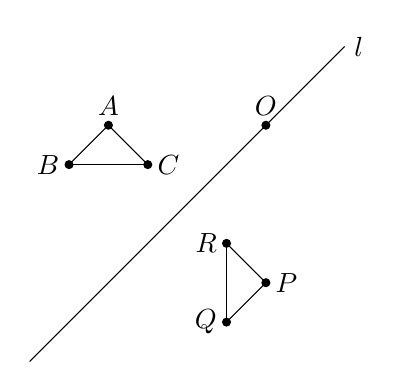
\begin{tikzpicture}
		\draw (-2,-2) -- (2,2) node[right] {$l$};
		\draw (-1,1) -- (-1.5,.5);
		\draw (-1.5,.5) -- (-.5,.5);
		\draw (-.5,.5) -- (-1,1);
		\draw (1,-1) -- (.5,-1.5);
		\draw (.5,-1.5) -- (.5,-.5);
		\draw (.5,-.5) -- (1,-1);
		\draw[fill=black] (-1,1) circle (0.05) node[above] {$A$};
		\draw[fill=black] (-1.5,.5) circle (0.05) node[left] {$B$};
		\draw[fill=black] (-.5,.5) circle (0.05) node[right] {$C$};
		\draw[fill=black] (1,-1) circle (0.05) node[right] {$P$};
		\draw[fill=black] (.5,-1.5) circle (0.05) node[left] {$Q$};
		\draw[fill=black] (.5,-.5) circle (0.05) node[left] {$R$};
		\draw[fill=black] (1,1) circle (0.05) node[above] {$O$};
	% line reflection
	\end{tikzpicture} 
	& 	
	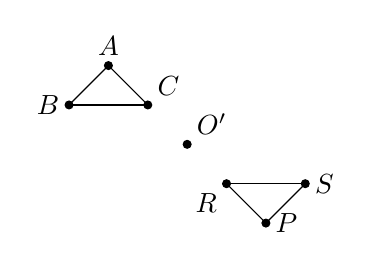
\begin{tikzpicture}
		\draw (-1,1) -- (-1.5,.5);
		\draw (-1.5,.5) -- (-.5,.5);
		\draw (-.5,.5) -- (-1,1);
		\draw (1,-1) -- (1.5,-.5);
		\draw (1.5,-.5) -- (.5,-.5);
		\draw (.5,-.5) -- (1,-1);
		\draw[fill=black] (0,0) circle (0.05) node[above right] {$O'$};
		\draw[fill=black] (-1,1) circle (0.05) node[above] {$A$};
		\draw[fill=black] (-1.5,.5) circle (0.05) node[left] {$B$};
		\draw[fill=black] (-.5,.5) circle (0.05) node[above right] {$C$};
		\draw[fill=black] (1,-1) circle (0.05) node[right] {$P$};
		\draw[fill=black] (1.5,-.5) circle (0.05) node[right] {$S$};
		\draw[fill=black] (.5,-.5) circle (0.05) node[below left] {$R$};
	% point reflection
	\end{tikzpicture}   \\
Line reflection about line $l$. & Point reflection about point $O'$. \\
& \\
\end{tabular}
\end{center}

Let $F$ be some real, ordered field. The coefficients of our linear fractional transformations will come from $F$. We begin with a notion inspired by Euclidean geometry: that both point reflections and line reflections should be of order two (as demonstrated above by the Euclidean reflections). That is, we want the composition of a transformation upon itself to yield the identity transformation. We first establish two lemmas. 

\begin{lemma} 
	The composition of linear fractional transformations corresponds to the multiplication of their respective matrix encodings.
\end{lemma}

\begin{proof} 
	Appeal to Theorem \ref{thm:function_correspondence} and Corollary \ref{thm:isomorphism}. (possibly want to flesh this out or make it less lemmay)
\end{proof}	
	
\begin{lemma}
	If $M_f$ is a matrix that encodes some linear fractional transformation $f$ of order two with coefficients in a field $F$, then we must have that $M_f^2 = \lambda I$ for some constant $\lambda \in F$, where $I$ is the usual $2 \times 2$ identity matrix. 
\end{lemma}

\begin{proof}
	Because $f$ is of order two, by definition we must have that $f \circ f$ is the identity function. In terms of matrices, by Lemma 3.1 we must then have that $M_f^2$ yields the identity of $PGL(2\ttc F)$\footnote{See \ref{thm:PGL2F} in Appendix \ref{appendixC} for the definition of $PGL(2\ttc F)$}. That is, we must have that $M_f^2 = \lambda I$ for some $\lambda \in F$.
\end{proof}

\begin{lemma}
	If $f$ is a linear fractional transformation and $M_f$ is the matrix encoding $f$, then we must have that $\det(M_f) \neq 0$.
\end{lemma}

\begin{proof}
	Suppose that for each $z \in \C$, $f$ is given by $f(z) = \frac{az+b}{cz+d}$ for some $a\ttc b\ttc c\ttc d \in F$. We have by (1) that $ad-bc \neq 0$. Thus, since $\det M_f = ad-bc$, we must have that $\det M_f \neq 0$ as well.
\end{proof}

\begin{theorem}
If $M$ is a matrix encoding some linear fractional transformation $f$, then $f$ is of order two under matrix multiplication if and only if $\Tr(M) = 0$ or $M = \lambda I$ for some $\lambda \in F$.\footnote{That is, $\lambda I$ is some representative of the identity coset of $PGL(2\ttc F)$.}
\end{theorem}

\begin{proof}
Let $M$ be a matrix that encodes a linear fractional transformation of order two. By Lemma 3.2, we must have that $M^2 = \lambda I$ for some constant $\lambda \in F$, where $I$ is the usual $2 \times 2$ identity matrix. In this case, we want to have that 
	\[
		\stanlftmat \stanlftmat = \lambda \lftmat{1}{0}{0}{1}
	\]
for some $\lambda \in F$. Expanding this further, we see that we must have 
	\[
		\lftmat{a^2 + bc}{b(a+d)}{c(a+d)}{bc+d^2} =  \lftmat{\lambda}{0}{0}{\lambda}
	\]
Looking at the upper-right and lower-left entries in the two above matrices, we see that $M^2 = \lambda I$ can hold if $a + d = 0$ or if $b = c = 0$. We consider these two cases in turn.

If $a + d = 0$, then by definition we have that $\Tr(M) = 0$.

\todo{[LG] i hate the visuals of it, but should we do this as matrices rather than straight algebra? I think it's fine. This is only one paragraph.} On the other hand, if $b = c = 0$, then it remains to ensure that $a^2 + bc = \lambda$ (the upper-left entries of the above matrices) and that $bc + d^2 = \lambda$ (the lower-right entries). Because we know that $b = c = 0$, we can simplify to see that $a^2 = \lambda$ and that $d^2 = \lambda$. Thus we know that $a = -d$ or that $a = d$. In the first case, $a = -d$ implies that $a + d = 0$, whence $\Tr(M) = 0$. If $a = d$, then $M$ is of the form 
\[\lftmat{a}{0}{0}{a}\]
for some $a \in F$. That is, $M$ is of the form $\lambda I$ if we take $\lambda = a$. 

For the other direction, first suppose that $M$ is a matrix with trace 0. Then
\[M = \lftmat{a}{b}{c}{-a}\]
for some $a \ttc b \ttc c \in F$. Notice that
\begin{align*}
M^2 & = \lftmat{a}{b}{c}{-a} \lftmat{a}{b}{c}{-a} \\[2ex]
& = \lftmat{a^2+bc}{ab - ba}{ca - ac}{cb+a^2} \\[2ex]
& = \lftmat{a^2+bc}{0}{0}{a^2 + bc}
\end{align*}
Therefore $M^2 = \lambda I$ if we take $\lambda = a^2 + bc$.

Finally, suppose that $M = \gamma I$ for some $\gamma \in F$. Then
\begin{align*}
M^2 & = \lftmat{\gamma}{0}{0}{\gamma} \lftmat{\gamma}{0}{0}{\gamma} \\[2ex]
& = \lftmat{\gamma^2}{0}{0}{\gamma^2}
\end{align*}
It follows that $M^2 = \lambda I$ if we take $\lambda = \gamma^2$.
\end{proof}

Now, recall by Lemma 3.3 that no linear fractional transformation can be encoded in a matrix with determinant 0. Thus we may only work with matrices whose determinants are either positive or negative. Guggenheimer encodes point reflections in matrices with positive determinant and line reflections in matrices with negative determinant. 

\noindent\todo{[AB][LG] make sure this all makes sense after LGdefines hyperbolic actions and clarifies where the disk lies}
Let $(x \ttc y)$ be a point in the \poincare disk. Then, for the matrix encoding the hyperbolic point reflection over $(x \ttc y)$ to satisfy $\Tr(M) = 0$ and $\det M = -(y^2 - x) > 0$, we say that $M$ is of the form
\begin{equation} 
	\lambda \stanpointmat \text{ where } \lambda \in F \text{ and } x > y^2. 
\end{equation}	
As mentioned, we choose to associate each point reflection with a unique point in the disk. It follows that the points in our \poincare disk are given by those points $(x \ttc y) \in F^2$ inside the convex domain of the parabola $x = y^2$.

It is important to remember that we are not mapping this parabola to the unit disk; we are instead using this parabola to define three disjoint subsets of $F^2$. In particular, the points in $F^2$ contained in the convex domain defined by the parabola $x=y^2$ correspond to the interior of the \poincare disk, those in $F^2$ that lie on the parabola $x=y^2$ correspond to the \poincare disk itself, and those neither inside nor on the parabola $x=y^2$ correspond to points outside the \poincare disk.

Next, we define $F_*$ to be the extension of $F$ by $\infty$ as usual\footnote{If we take $F = \R$, then we follow the convention set forth in \cite{shuman_infinity}. However, it is unclear how to do this in an arbitrary field. Guggenheimer does not address this complication.}. We define an end of our geometry to be the points on our parabola, namely those pairs $(x \ttc y) \in F_*^2$ where $y = x^2$. We follow Guggenheimer in simply claiming that the end $\specialend$ is of particular interest to us in our classification of line reflections. In particular, the reflection over a line $l$ given by $(l_1\ttc l_2)$ that does not pass through the end $\specialend$ can be encoded in the matrix
\[\stanlinenoendmat\]
If the line $l$ given by $(l_1\ttc l_2)$ does pass through the end $\specialend$, then the reflection over $l$ can be given by the following matrix:
\[
	\stanlineendmat
\]

Following Guggenheimer's decision, we will uniquely associate all lines $l$ with their reflections, just as we did with point reflections. We now discuss the forms that our two types of line reflections must take. \\
\todo{[AB] make Karen's comments from bottom of pg.~10 more explicit?}

\begin{theorem}The equation of a line in $F_*^2$ not passing through the end $\specialend$ must be of the form \begin{equation}
	x - 2l_2y + l_1  = 0.
\end{equation} 
where $l_1$ and $l_2$ are in $F_*$; $x \in F_*$; and $y \in F_*$.
\end{theorem}

\begin{proof}
Notice that if a point $P$ is on a line $l$, then by our geometric intuition, the $f_l$ fixes $P$. Regarding our point $P$ and line $l$ as their respective reflections, we then have that $f_l(P) = P$ if point $P$ is on line $l$. For the same reason, we have that $M_{f_l} M_{f_P} M_{f_l}\inv = M_{f_P}$, whence $M_{f_l} M_{f_P} = M_{f_P} M_{f_l}$. We will first consider this in terms of matrices for lines not passing through the end $\specialend$. We have the following\footnote{$M_{f_l} M_{f_P}$ is a representative of $M_{f_P} M_{f_l}$, hence the $\lambda$.}:
\begin{equation} 
\stanlinenoendmat\stanpointmat \spceq \lambda \stanpointmat\stanlinenoendmat
\end{equation}	
Expanding, we see that we must have
	\[
		\lftmat{-l_2y+l_1}{-l_2x+l_1y}{y-l_2}{x-l_2y} \spceq \lambda \lftmat{-l_2y+x}{-l_1y+l_2x}{l_2-y}{l_1-l_2y}
	\]
Looking at the lower-left corner of our matrices, we see that we must have $\lambda = -1$ since $y - l_2 = -1(l_2 - y)$. If we then consider the upper-left corner, we must have that $-l_2y + l_1 = -1(-l_2y + x)$. Simplifying, we see that equations of lines not passing through the end $\specialend$ must be of the form $x - 2l_2y + l_1  = 0$ as desired.
\end{proof}

\begin{theorem} The equation of a line in $F_*^2$ passing through the end $\specialend$ must be of the form 
\begin{equation}
	2y = l_1.
\end{equation} 
where $l_1$ and $y$ are elements of $F_*$.
\end{theorem}

\begin{proof} If $l$ is a line passing through the end $\specialend$ and $P$ is some point on $l$, we again have that $M_{f_l} M_{f_P} = M_{f_P} M_{f_l}$. Again realizing this in terms of matrices, we have that 
\begin{equation} 
	\stanlineendmat\stanpointmat \spceq \lambda \stanpointmat\stanlineendmat
\end{equation}	
We again expand to see that 
	\[
		\lftmat{-y+l_1}{-x+l_1y}{-1}{-y} \spceq \lambda \lftmat{-y}{-l_1y+x}{1}{l_1-y}
	\]
By considering the lower-left entry into these matrices we see that $\lambda = -1$. We can now find the general form of such lines by seeing from the upper-left entries that $-y+l_1 = -y$. Simplified, our form is $2y = l_1$. 
\end{proof}

With this in hand, we now develop and visualize examples of these transformations with coefficients in the real ordered field $\R$. Then, motivated by Guggenheimer's claim that hyperbolic geometry can be derived along these lines if we instead take the coefficients of our linear fractional transformations from the complexified field $\fc$.



%%%%%%%%%%%%%%%%%%%%%%%%%%%%%%%%%%%%%%%%%%%%%%%%%%%%%%%%
\section{Examples in $F = \R$}

\hspace{10mm} We choose $\R$ to be our real, ordered field as called for in Guggenheimer's paper and go forth to visualize some examples of transformations in the \poincare disk. We work with two triangles\footnote{To define a triangle, we take three points in the disk and connect them with hyperbolic lines.} and two points about which each of them will be reflected\footnote{To reflect a triangle over a point $P$, we apply $f_P$ to each of its three vertices and then ``redraw" the edges. See Appendix D for the code used.}. Triangle $T_1$ is given by the points $A_1 = 0 + 0i$, $B_1 = 1 + 0i$, and $C_1 = 0 + 1i$. Triangle $T_2$ is given by the points $A_2 = 3 + 5i$, $B_2 = -4 + 4i$, and $C_2 = 0.2 - 2i$. The points about which we will perform our reflections are $X = (2, -1)$ and $Y = (2, 1)$.

More concretely, we take our points $X$ and $Y$ and encode $f_X$ and $f_Y$ (the reflection functions over $X$ and $Y$ respectively) in matrices $M_{f_X}$ and $M_{f_Y}$. In particular, by (1) we have that 
\[M_{f_X} = \lftmat{-1}{2}{-1}{1} \text{ and } M_{f_Y} = \pointmat{2}{1}.\]
Notice that for simplicity, in both of these cases we chose $\lambda = 1$ \todo{[LG] do we have to address this any further? I don't think so but it's worth asking.} Now, we know by (2) that for all $z \in \C$, $f_X$ and $f_Y$ are given by $f_X(z) = \frac{-x+2}{-x+1}$ and $f_Y(z) = \frac{x+2}{-x-1}$ respectively. Thus, to apply these transformations to a point \todo{[LG] WAIT, SO DO WE PUT THE POINT IN THE DISK FIRST AND THEN TRANSFORM OR TRANSFORM AND THEN PUT IT IN THE DISK? CAN YOU FINISH THIS PART? WE'RE REALLY JUST MISSING A SENTENCE OR TWO}

As we consider these visualizations, recall the three types of points in the \poincare disk. Points in the interior of the disk are mapped from the convex domain given by the parabola $x = y^2$. Points outside the \poincare disk are strictly outside the domain given by $x = y^2$. The points on the \poincare disk -- those mapped from points lying on the parabola $x=y^2$ -- are called the ``ends" of our geometry.

Recall further that Guggenheimer distinguishes between line reflections defined by two different types of lines: those passing through the end $\specialend$ and those not passing through the end $\specialend$. Although we suspect that for a linear fractional transformation $f$ given by $z \mapsto \frac{az+b}{cz+d}$, the end $\specialend$ corresponds to the expression $f(\frac{-d}{c})$ (that is, division by zero), this is not addressed by Guggenheimer and thus we avoid lines of this type. Thus we are left to assume that the end $\specialend$ does not correspond to any of the points on the boundary of the \poincare disk. 

As a final point of clarification, in our diagrams it will always appear that our hyperbolic lines can be extended to pass through two ends (i.e. touch the edge of the \poincare disk in two places). However, these are the general ends of the \poincare disk -- those mapped from the parabola $x = y^2$ in $\R^2$ -- not the particular end $\specialend$. \todo{[AB][LG] make sure this makes sense with LG new info from intro}

Now, below are our diagrams. We made these diagrams using the Geogebra\footnote{\cite{geogebra_software}} visual algebra tool and the corresponding user-made hyperbolic geometry worksheet\footnote{\cite{hyperbolic_worksheet}}.

\iffalse
\begin{center}
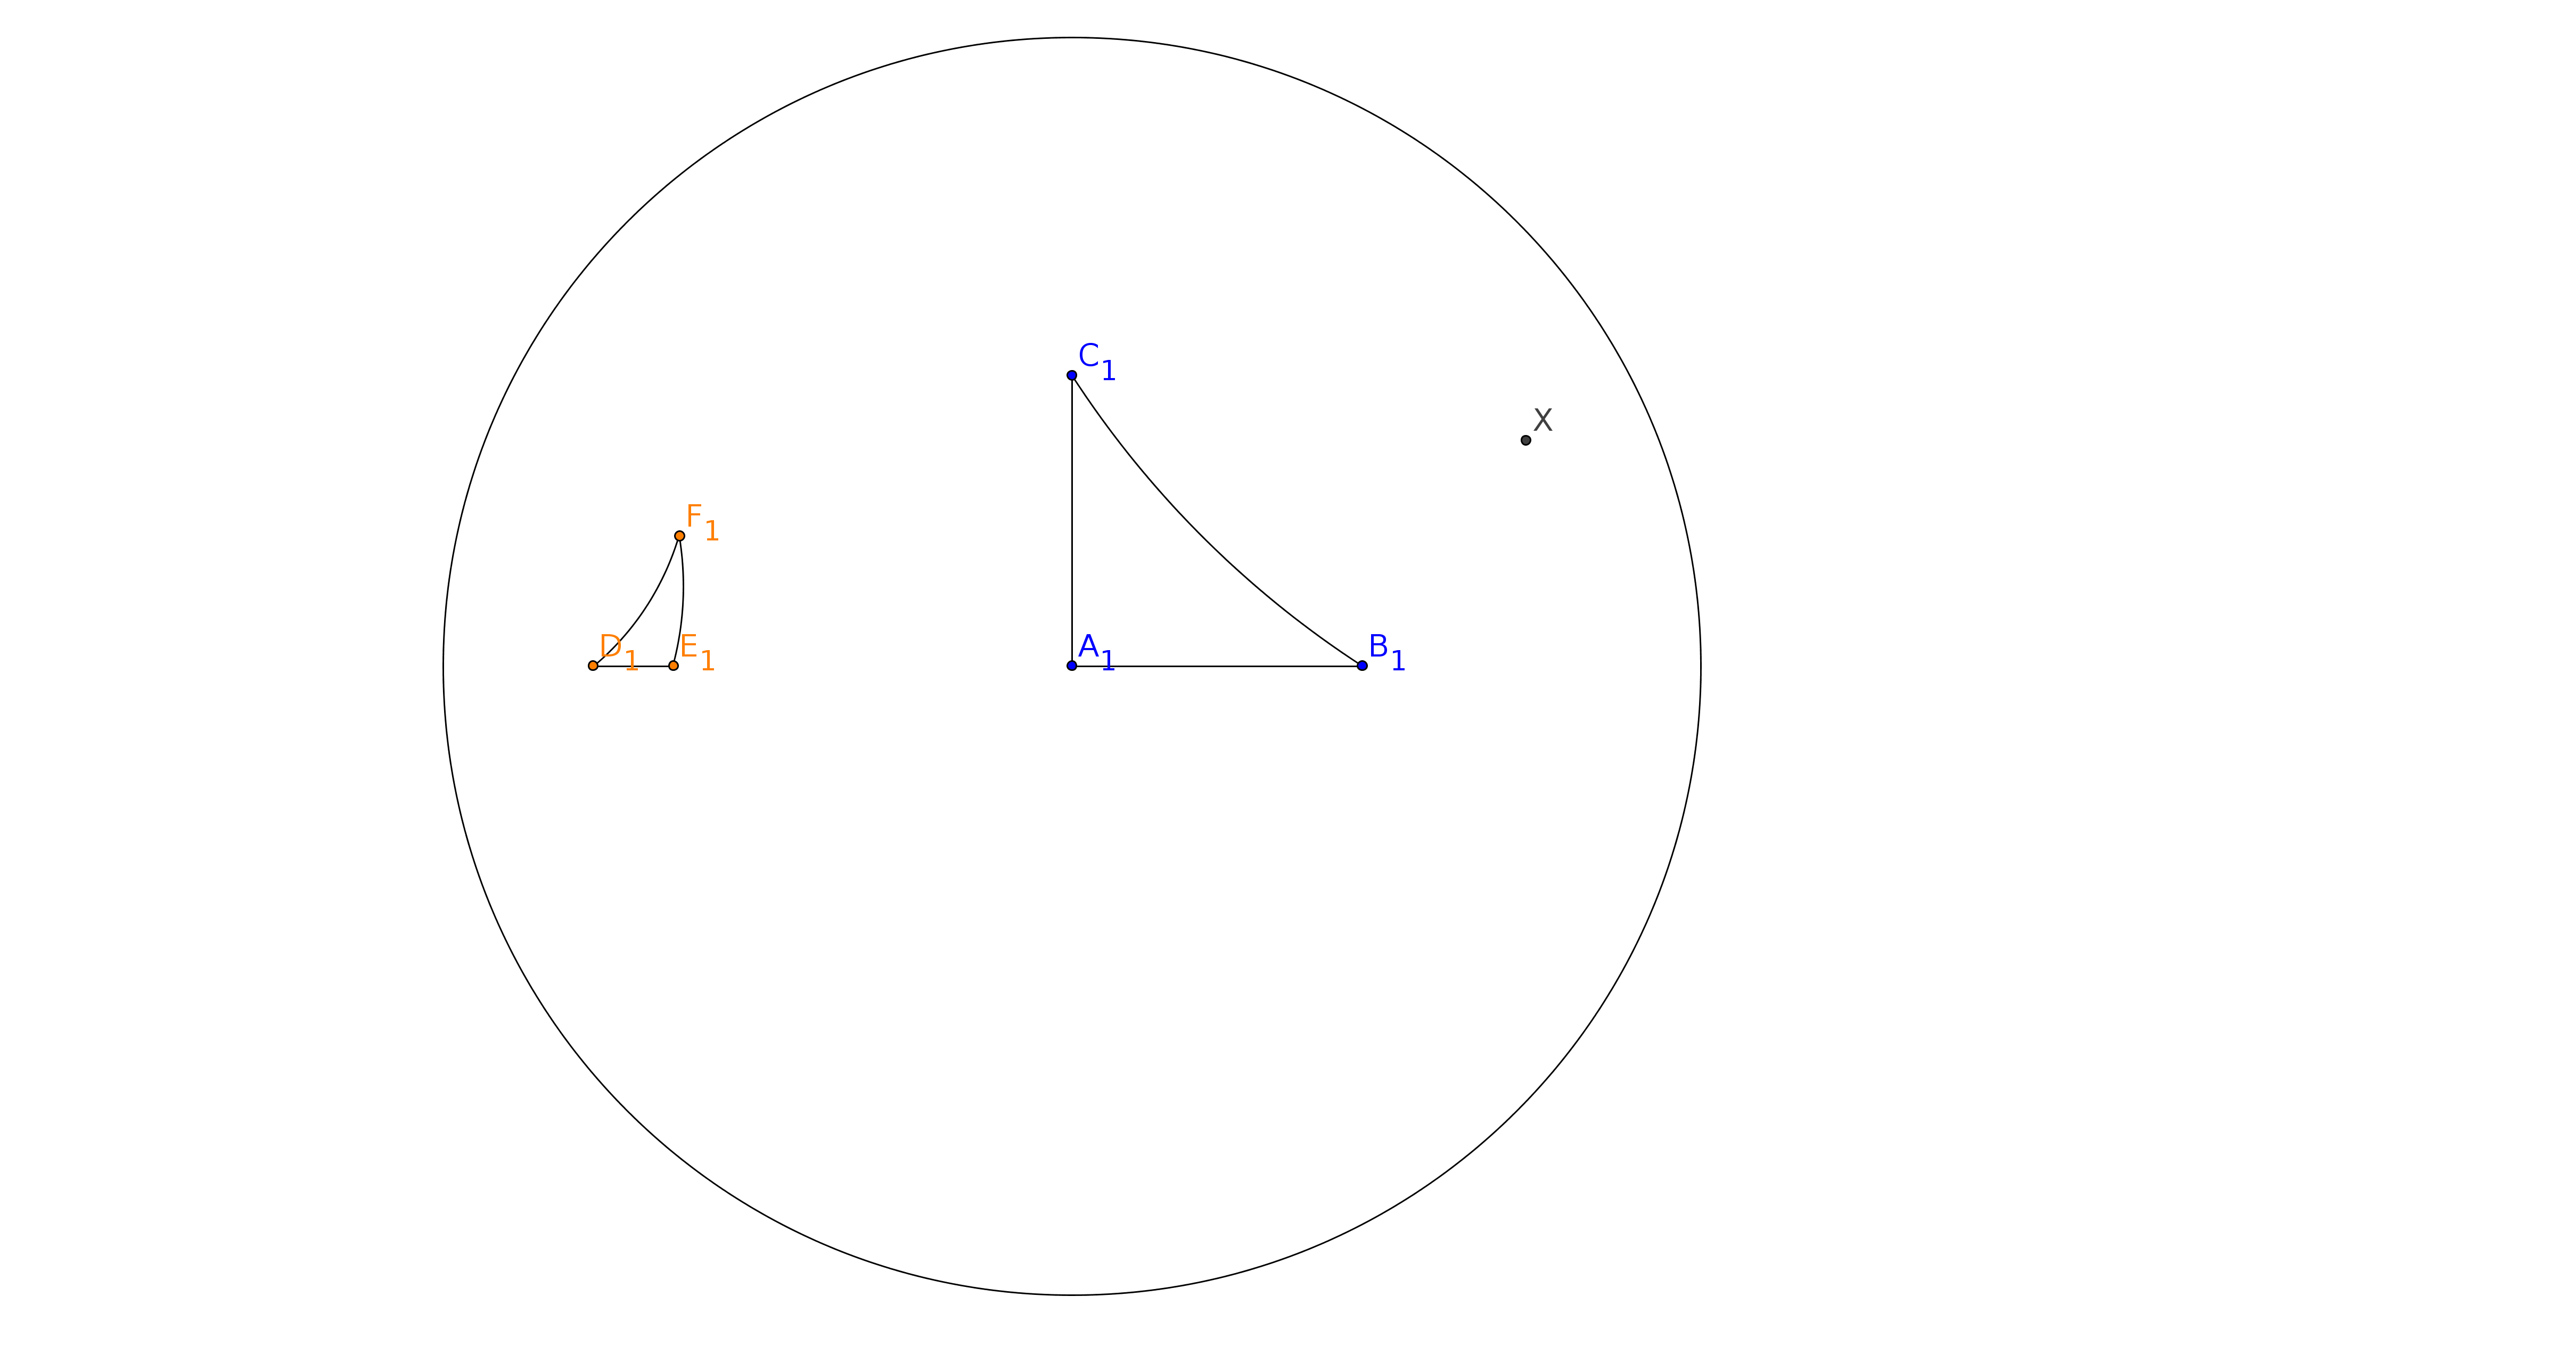
\includegraphics[width=160mm]{../images/t1_over_x.png} \\
Triangle $T_1$ reflected over point $X$ 
\[\]
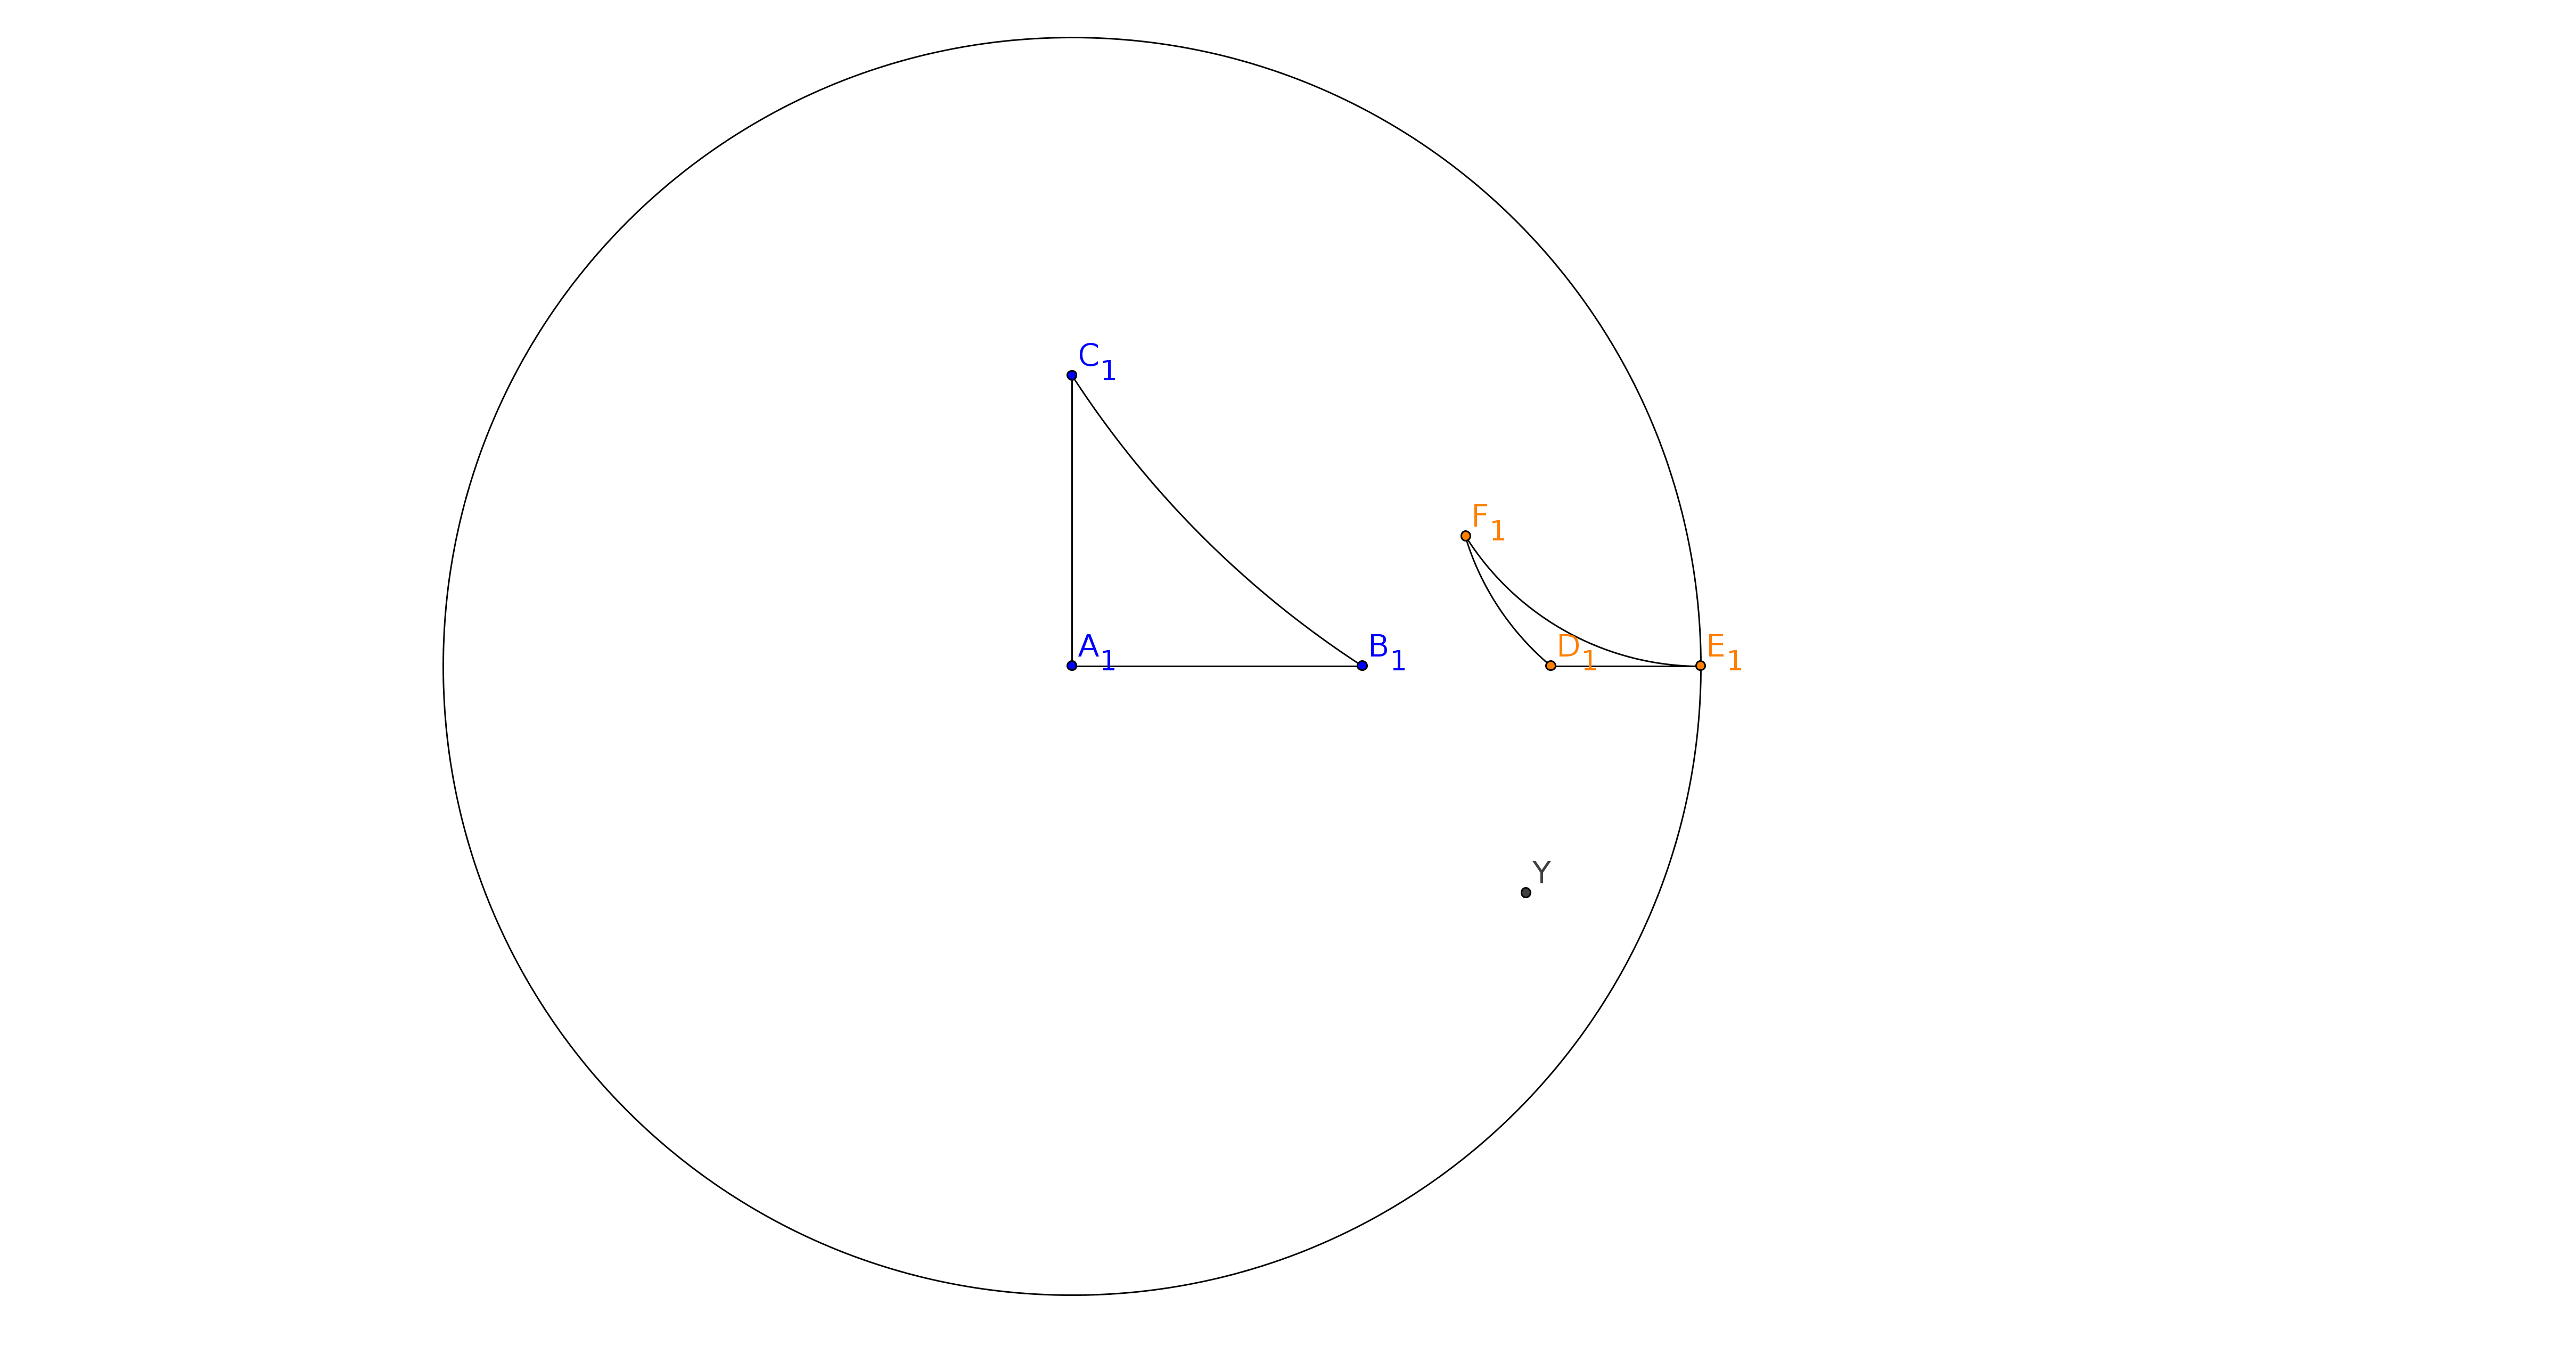
\includegraphics[width=160mm]{../images/t1_over_y.png} \\
Triangle $T_1$ reflected over point $Y$  
\[\]
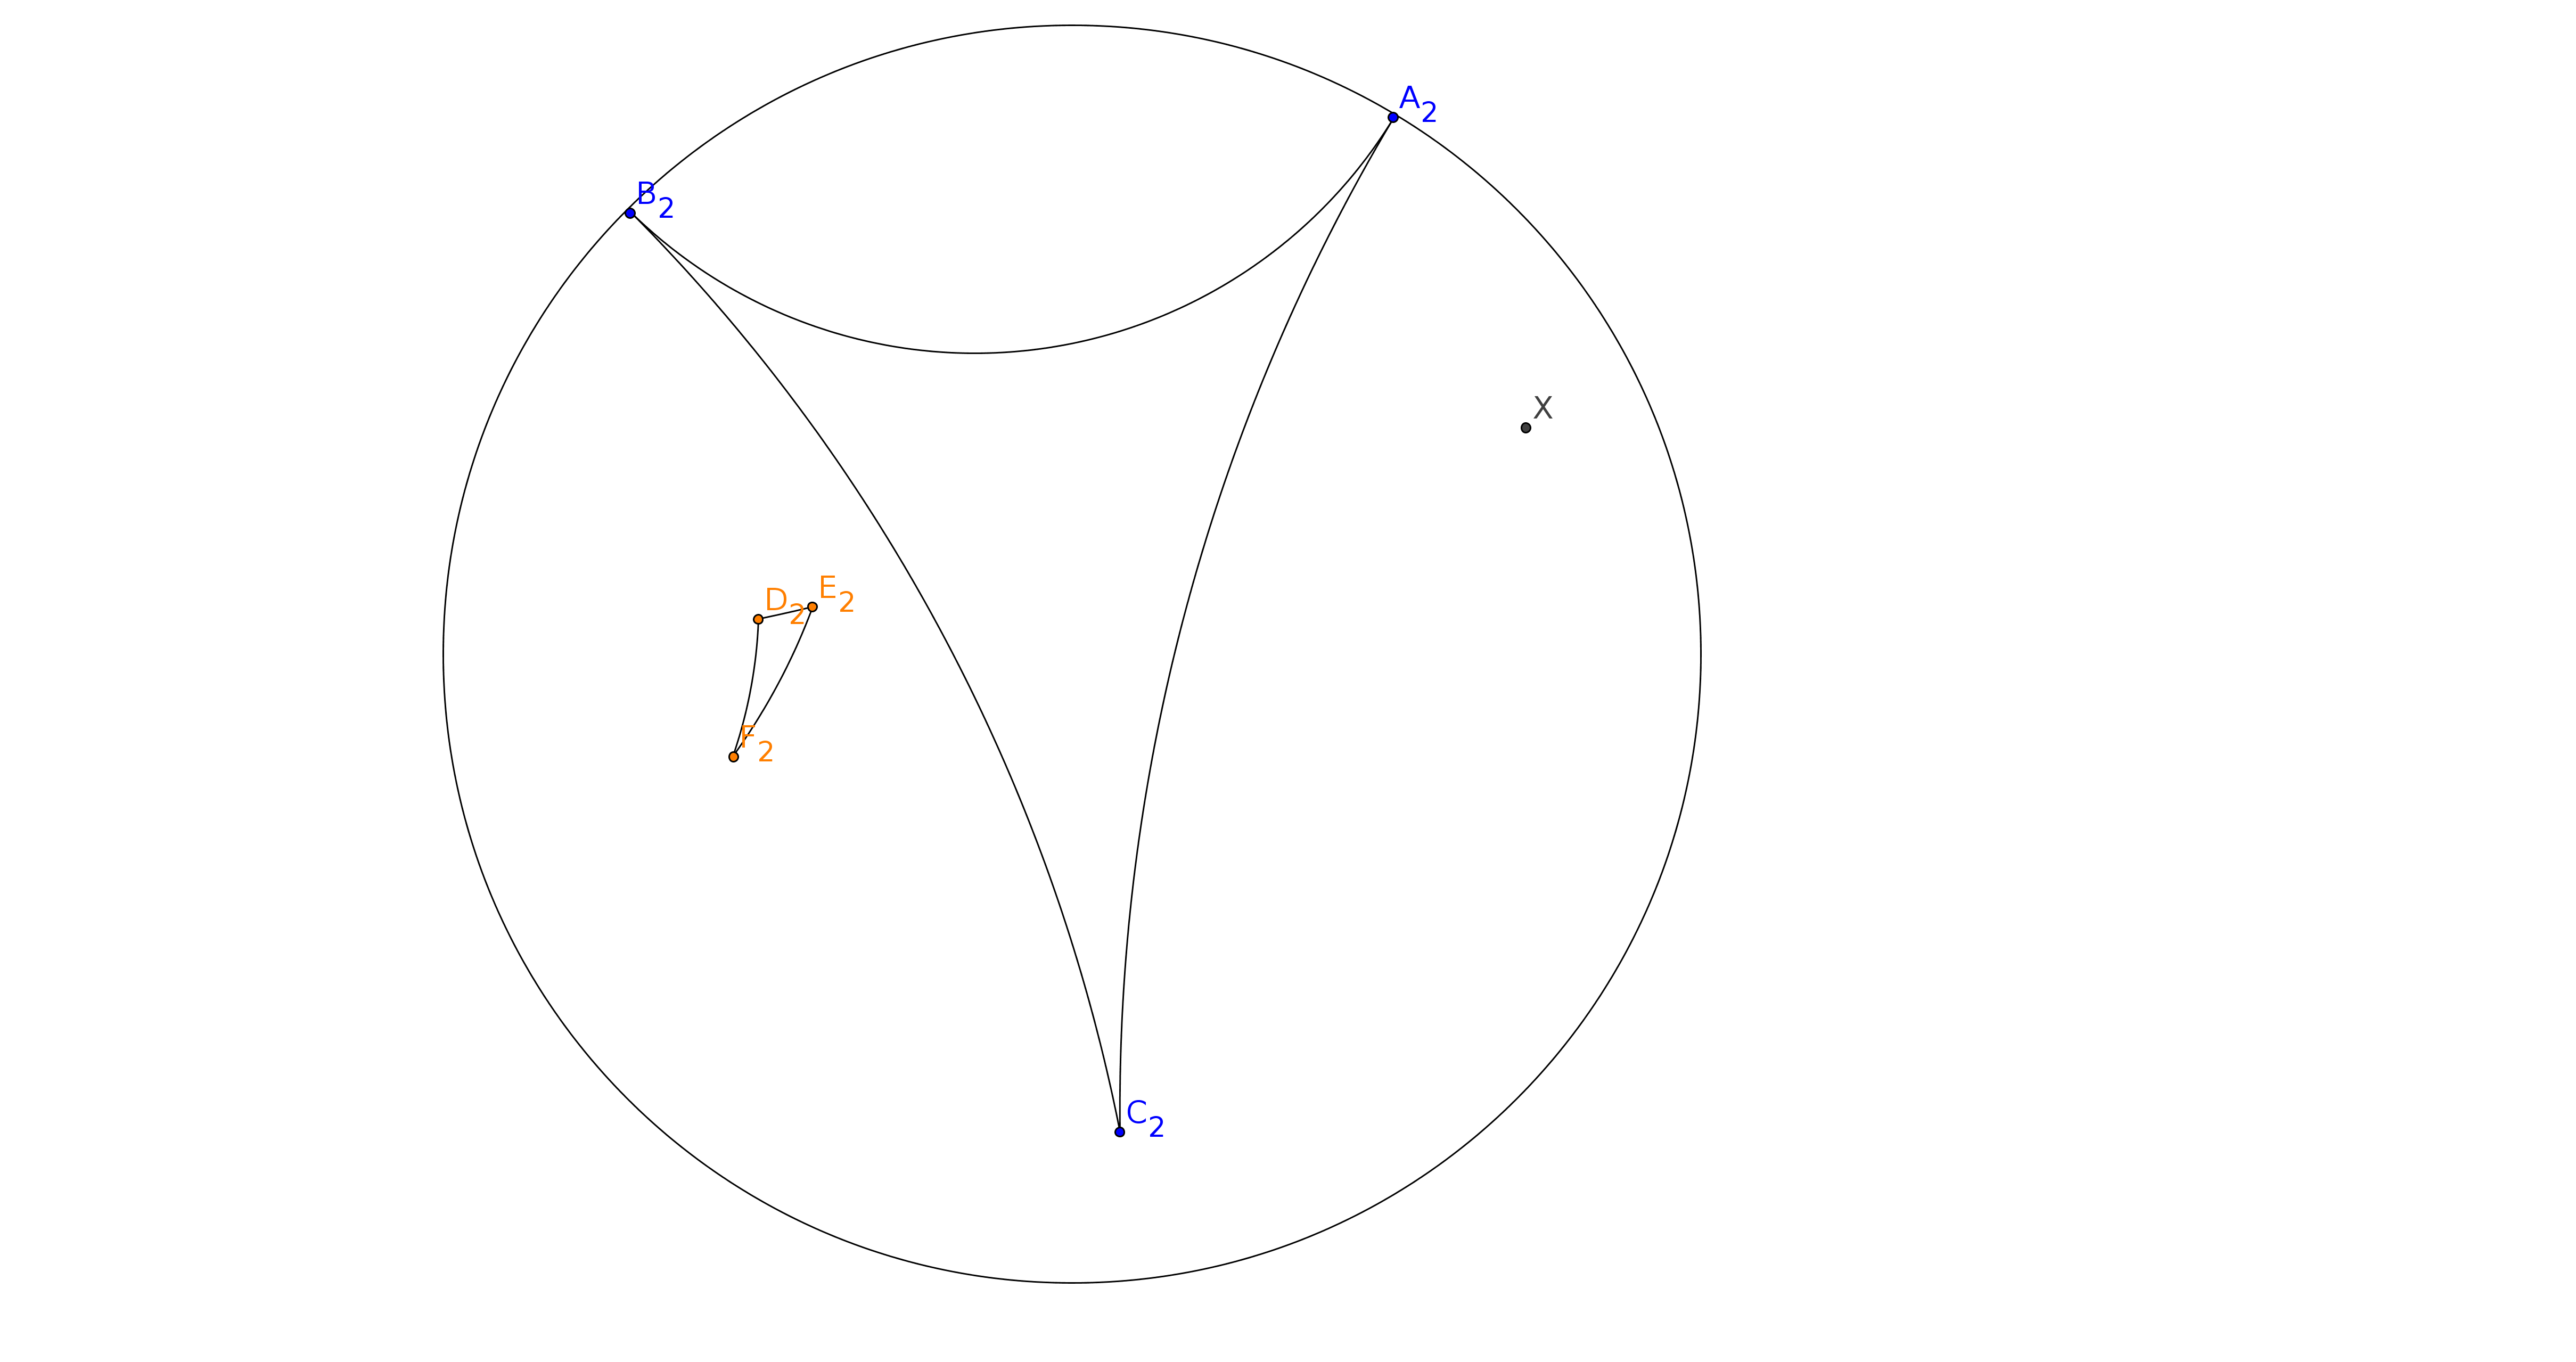
\includegraphics[width=160mm]{../images/t2_over_x.png} \\
Triangle $T_2$ reflected over point $X$
\[\]
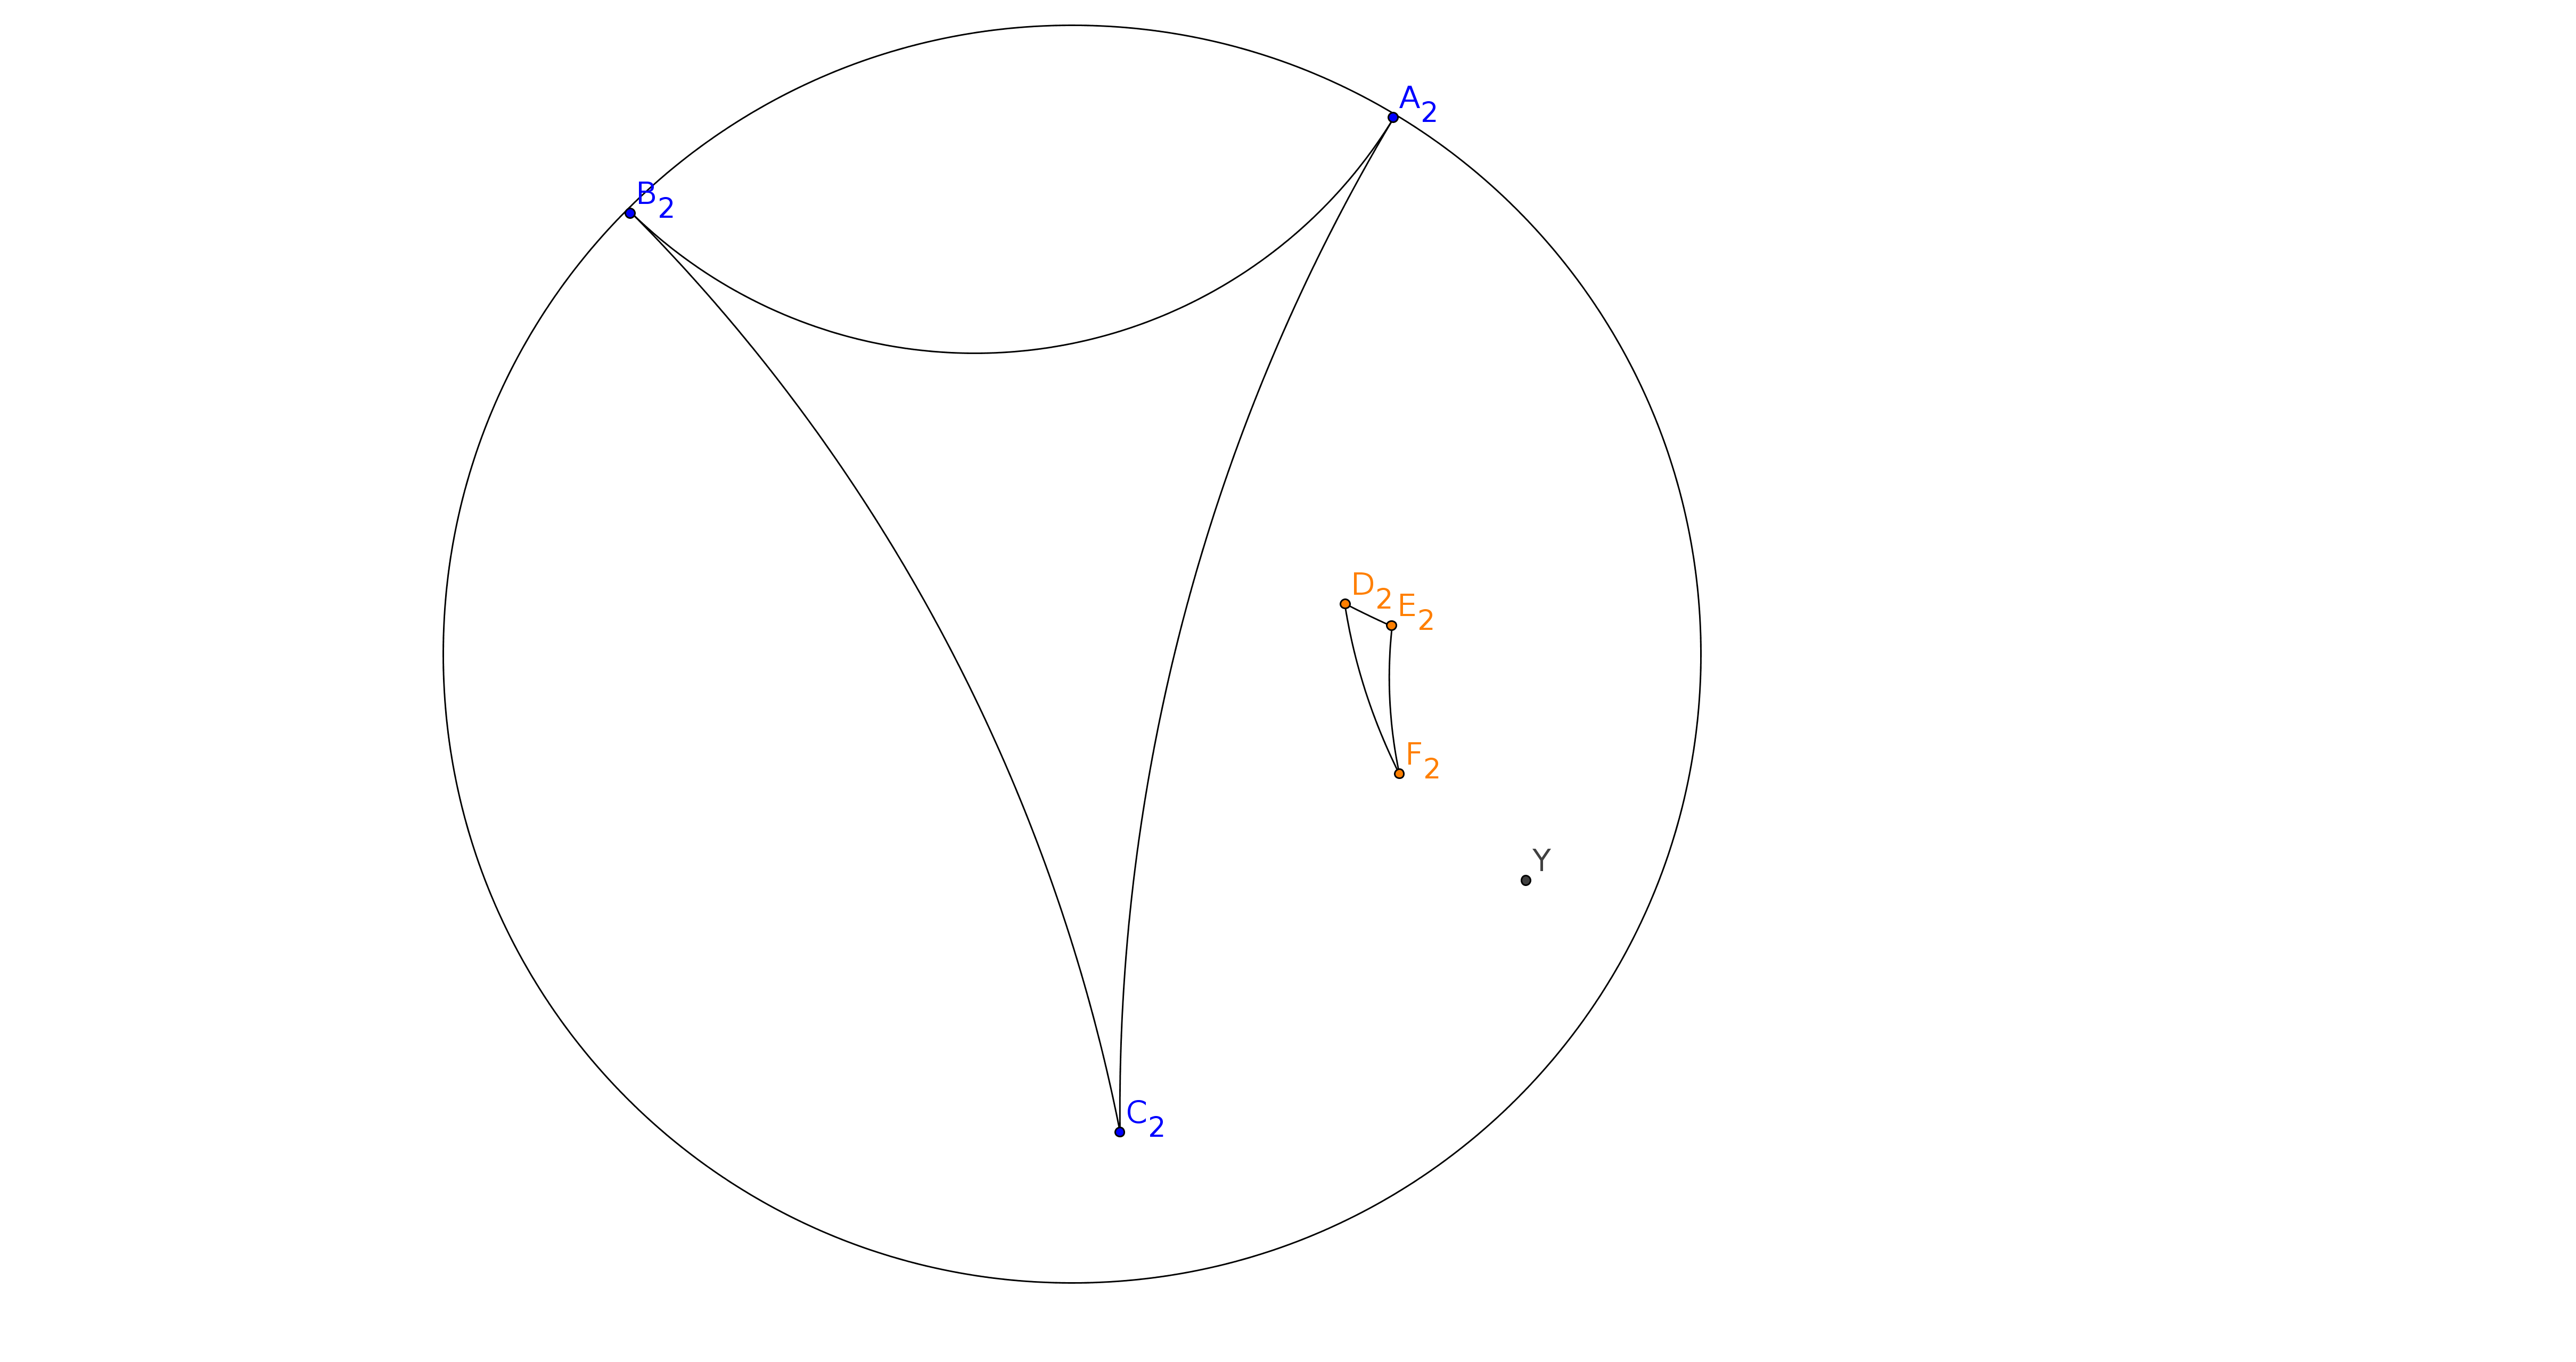
\includegraphics[width=160mm]{../images/t2_over_y.png} \\
Triangle $T_2$ reflected over point $Y$ 
\end{center}
\fi


From these diagrams we notice two oddities. For one, these point reflections look more like line reflections than they do point reflections. That is, the triangles seem to be ``reflected" and ``stretched" rather than simply ``rotated." Also, it is unclear from these diagrams why we restricted our choice of points to those from the convex domain defined by the parabola $x = y^2$. We now discuss these issues and their implications in turn.

As mentioned, these point reflections match an intuitive conception of a line reflection more than they do a point reflection. A closer look at the matrix encodings of point reflections and line reflections sheds light on this. 

\begin{theorem}
By Guggenheimer's definitions, all line reflections can be encoded as point reflections. 
\end{theorem}

\begin{proof}
Suppose that we have a line reflection $f_l$ given by $l = (l_1, l_2)$. We then encode the corresponding reflection in the matrix 
\[ M_{f_l} := \stanlinenoendmat. \]
To show that $f_l$ can be encoded as a point reflection, notice that 
\[ -1 \cdot \stanlinenoendmat = \lftmat{l_2}{l_1}{-1}{-l_2}.\]
Notice further that this matrix takes the form of a point reflection about $l = (l_1, l_2)$ if we set $\lambda = -1$. It follows that all line reflections can indeed be encoded as point reflections.
\end{proof}

Therefore the ``distinction" between line reflections and point reflections as put forth by Guggenheimer is indeed as arbitrary as it originally seemed. 

A further issue with this distinction arises once we complexify $\R$ as suggested by Guggenheimer. Because $\R^{\C} = \C$ is not ordered, there is no way to compare the determinant of a matrix $M$ with entries in $\C$ to 0. This issue will occur in all complexified fields, as no complexified field can be ordered\footnote{[\cite{marsden_complex_book}, p.~6]}. Thus, Guggenheimer's distinction between line reflections and point reflections by the determinant of their corresponding matrices is arbitrary at best and entirely non-applicable at worst.

Another crucial element of Guggenheimer's geometry is rendered nonsensical once we begin to work with complexified fields. In particular, his insistence that points be taken from the convex domain defined by the parabola $x = y^2$ (hereafter referred to as $D$) has no meaning in fields that are not ordered.

However, there is no clear geometric motivation behind this choice anyway. To investigate this, we reflect triangles $T_1$ and $T_2$ as defined above over a new point $Z = (-2, 1)$, which does not satisfy the condition $x > y^2$. 

\iffalse
\begin{center}
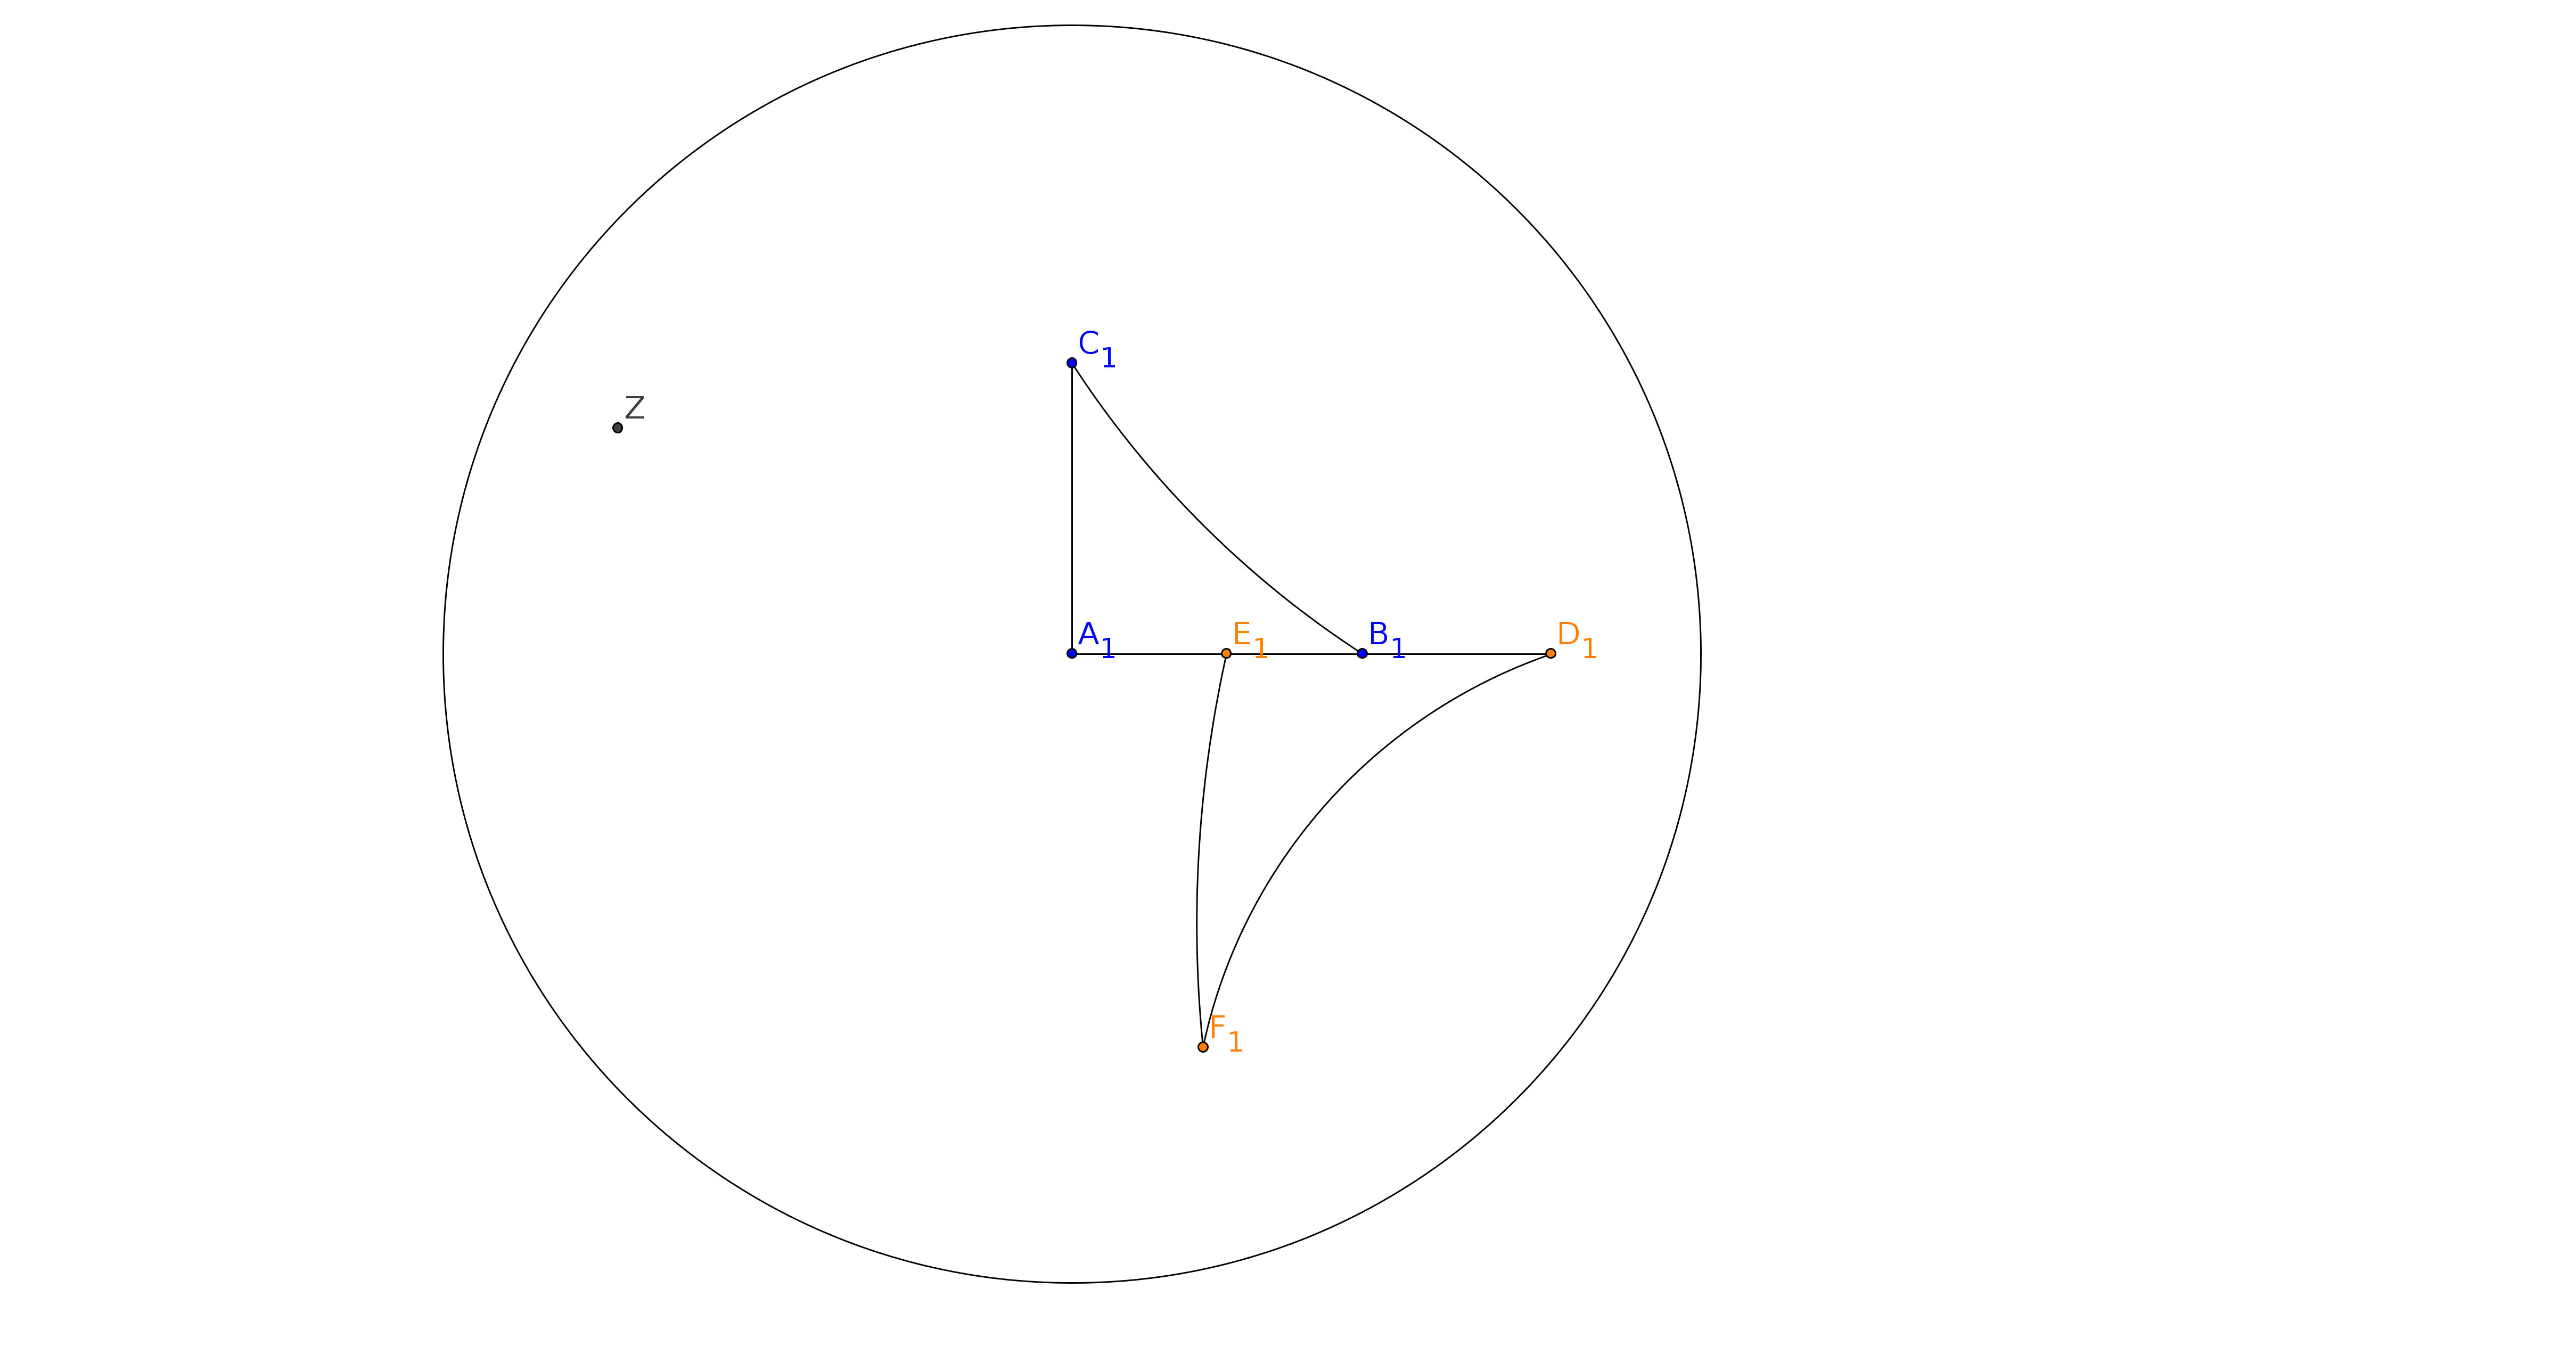
\includegraphics[width=165mm]{../images/t1_over_z.png} \\
Triangle $T_1$ reflected over point $Z$
\[\]
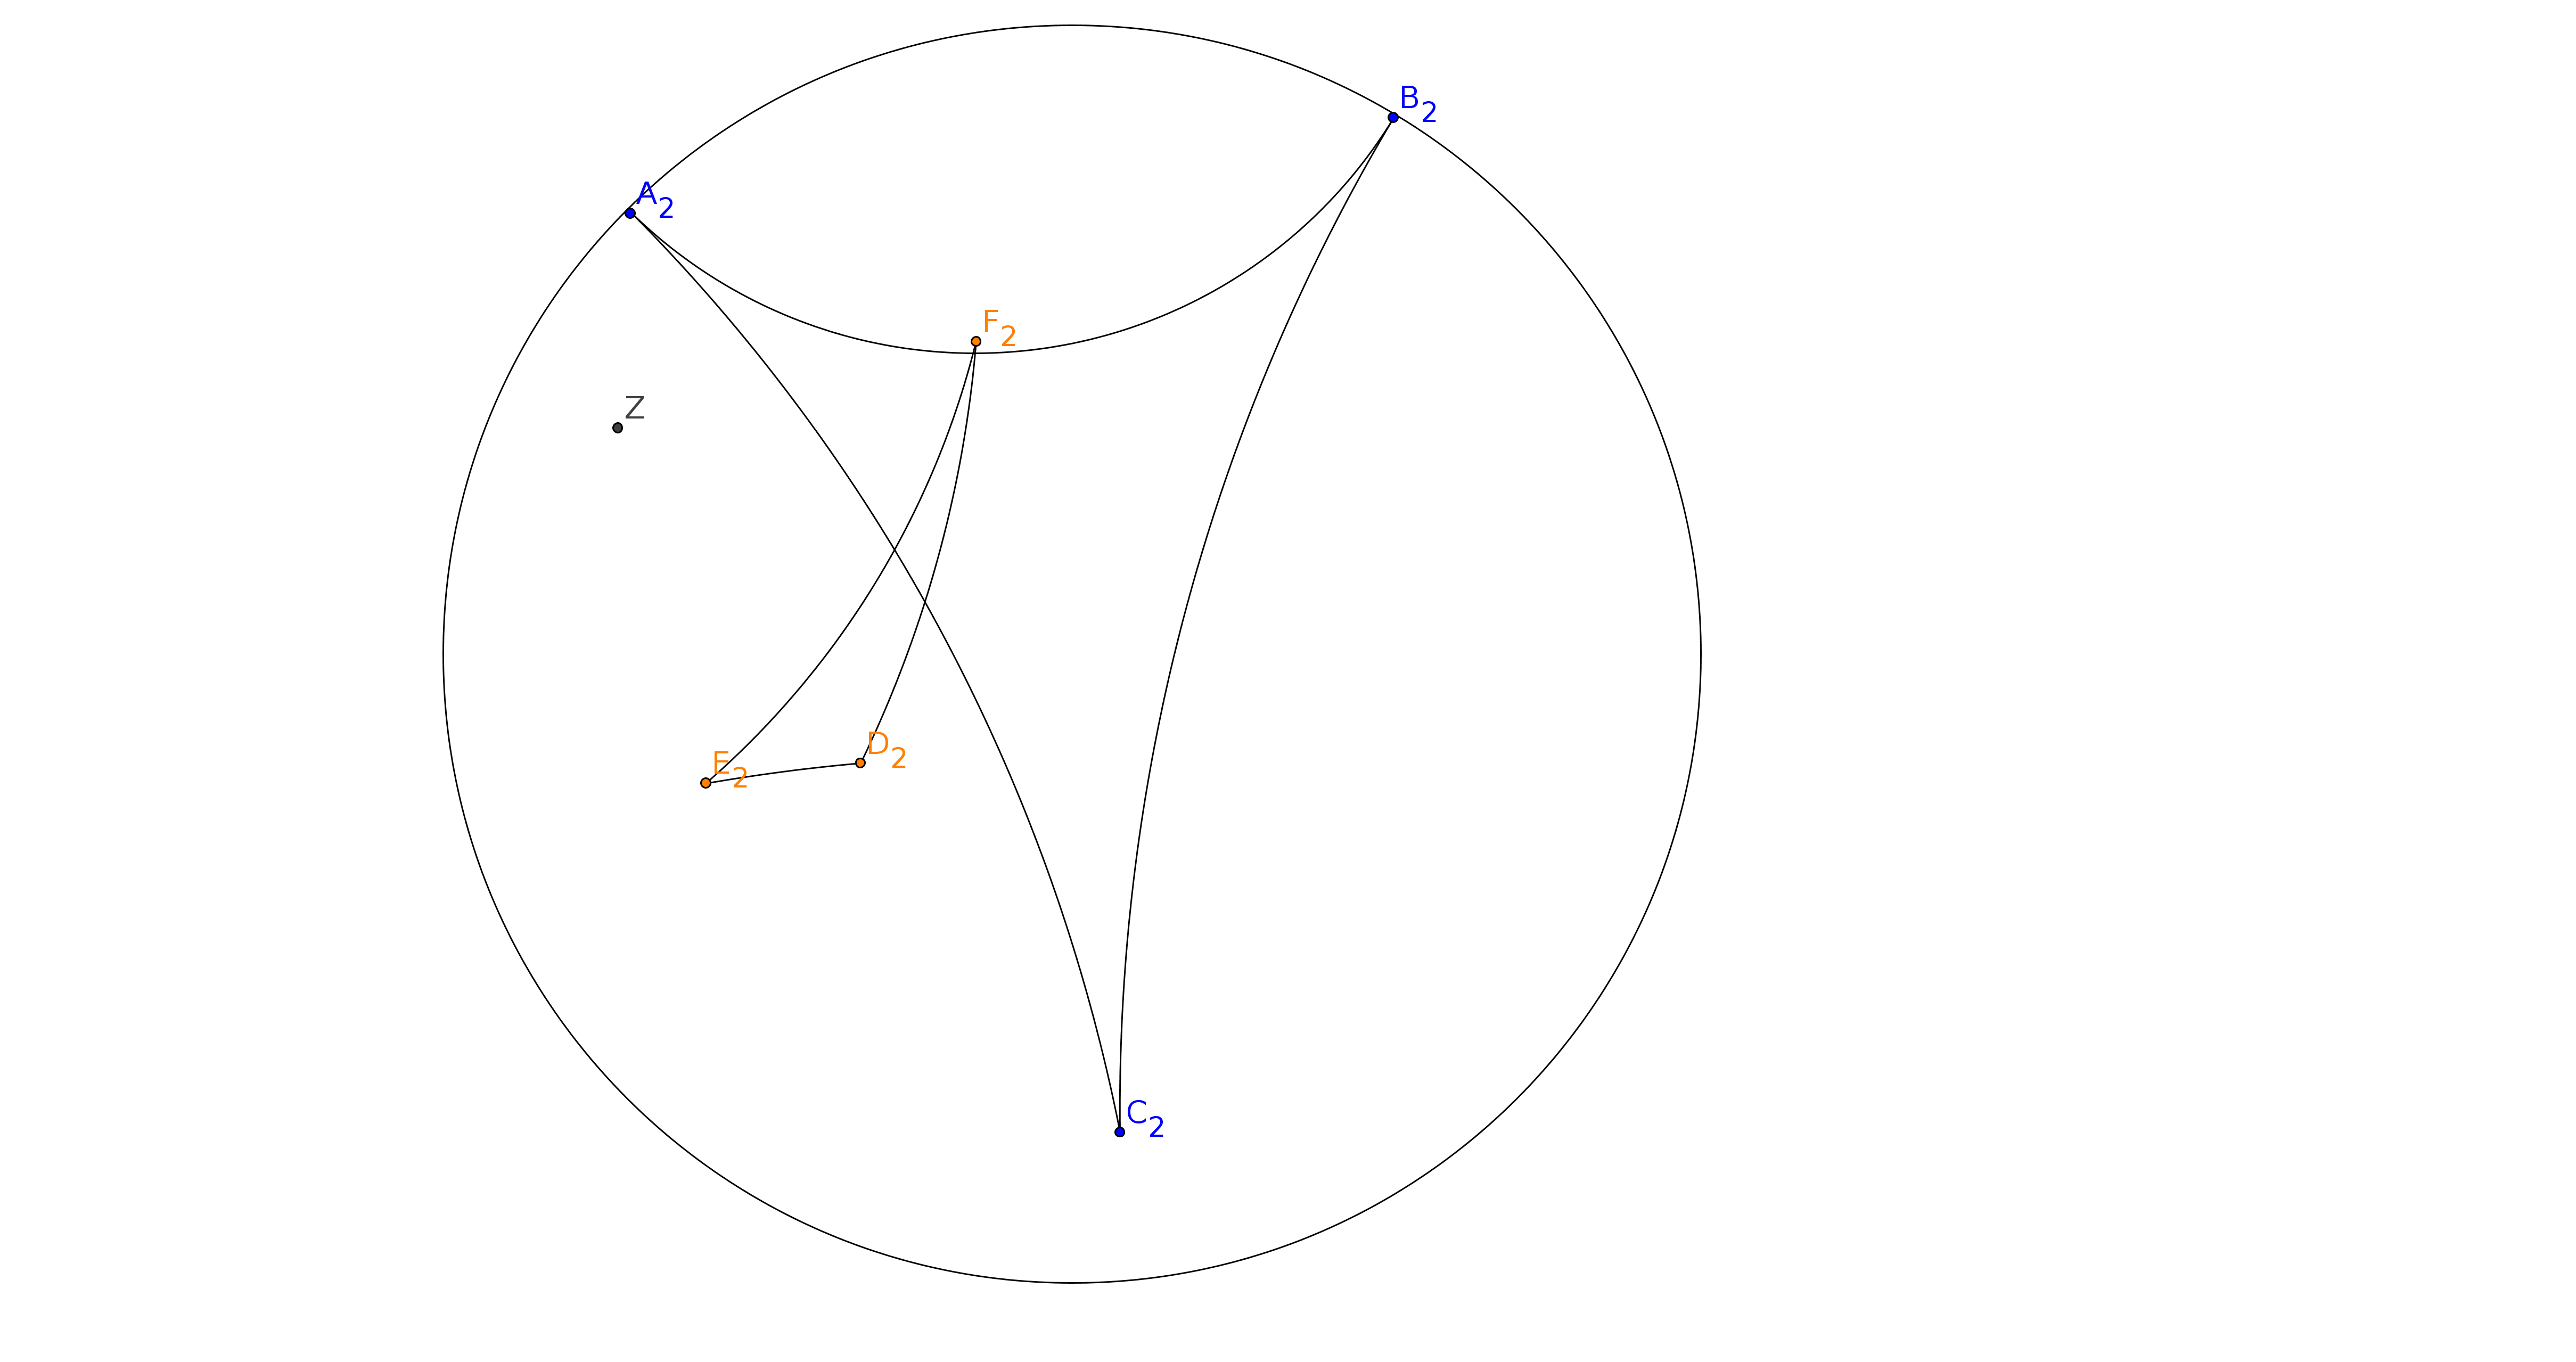
\includegraphics[width=165mm]{../images/t2_over_z.png} \\
Triangle $T_2$ reflected over point $Z$  
\end{center}
\fi

Although Guggenheimer would claim that it is invalid to reflect points over $Z$ since $Z \notin D$, these reflections function similarly to those given by points within $D$. Thus, his restriction that points defining reflections must be contained in $D$ is entirely unnecessary. 

In summary, we find three problems with Guggenheimer's geometry. For one, his algebraic distinction between line reflections and point reflections appears to be largely unimportant from a geometric perspective. Similarly, his imposition of the domain $D$ has neither algebraic motivation nor geometric justification. Finally, these two crucial elements to Guggenheimer's geometry are not even applicable to fields that are unordered. It is therefore impossible to substantiate his claim that this geometry can be developed in complexified fields.

%%%%%%%%%%%%%%%%%%%%%%%%%%%%%%%%%%%%%%%%%%%%%%%%%%%%%%%%
\newpage
\begin{appendices}
\section{From $\R^2$ to the \poincare Disk} \label{appendixA}
\noindent\todo{[AB][LG] ``You are mapping $\R^2$"}

Let $\Gamma$ be the \poincare disk. Suppose that we wish to translate the Euclidean point $A$, pictured arbitrarily below, to its equivalent point $A'$ in the \poincare disk.

\begin{center}
\begin{tikzpicture}[scale=.7]
\draw (0,0) circle (2.2cm) node[above left=1.5cm] {$\Gamma$};
\draw[fill=black] (2.2,2.2) circle (0.05) node[right] {$A$};
\end{tikzpicture}
\end{center}

We begin by constructing a line segment between $A$ and the origin $O$ and in order to find the Euclidean distance, $d_E$, between points $A$ and $O$.

\begin{center}
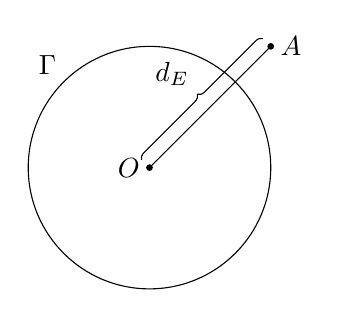
\begin{tikzpicture}[scale=.7]
\draw (0,0) circle (2.2cm) node[above left=1.5cm] {$\Gamma$};
\draw (0,0) -- (2.2,2.2);
\draw[fill=black] (0,0) circle (0.05) node[left] {$O$};
\draw[fill=black] (2.2,2.2) circle (0.05) node[right] {$A$};
\draw[decoration={brace,raise=4pt},decorate]
  (0,0) -- node[above left= 6pt] {$d_E$} (2.2,2.2);
\end{tikzpicture}
\end{center}

To construct the point $A'$, we want to find the radius $r$ in Euclidean distance of the circle whose hyperbolic distance from $O$ is $d_E$; $A'$ lies on this circle of radius $r$. In other words, if $d_H$ is the hyperbolic metric and $d_H(O,A') = d_E(O,A)$, then we want to find the circle, with radius $r\in\R$ centered at $O$, that contains $A'$. From \href{}{[source]} Theorem 9.1, we obtain the hyperbolic metric
\[
	d_H(O,A') = \ln\frac{1 + r}{1 - r}
\]
where $r\in\R$ is the radius of the circle we wish to draw. Let's call this new circle $\Delta$. Computing $r$, we find that
\[
	r = \frac{e^{d_H(O,A')} - 1}{e^{d_H(O,A')} + 1} =  \frac{e^{d_E(O,A)} - 1}{e^{d_E(O,A)} + 1}.
\]

Since $d_E(O,A)\in\R$, we conclude that $e^{d_E(O,A)} + 1 \neq 0$. Having computed $r$, we now draw the circle $\Delta$.

\begin{center}
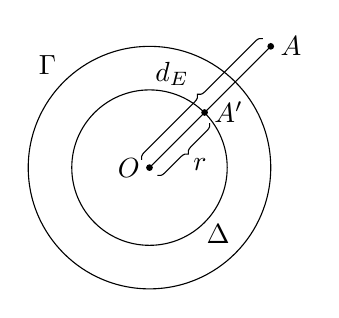
\begin{tikzpicture}[scale=.7]
\draw (0,0) circle (2.2cm) node[above left=1.5cm] {$\Gamma$};
\draw (0,0) circle (1.41cm) node[below right=.85cm] {$\Delta$};
\draw (0,0) -- (2.2,2.2);
\draw[fill=black] (0,0) circle (0.05) node[left] {$O$};
\draw[fill=black] (2.2,2.2) circle (0.05) node[right] {$A$};
\draw[fill=black] (1,1) circle (0.05) node[right] {$A'$};
\draw[decoration={brace,raise=4pt},decorate]
  (0,0) -- node[above left= 6pt] {$d_E$} (2.2,2.2);
\draw[decoration={brace,mirror,raise=4pt},decorate]
  (0,0) -- node[below right = 4pt] {$r$} (.95,.95);
\end{tikzpicture}
\end{center}

This point $A'$, the intersection between the line segment $\overline{OA}$ and $\Delta$, is the \poincare Disk-equivalent of our original point $A$.

Now if $B$ is a point on the line given by $OA$ along the ray $\overrightarrow{OA}$, our construction then maps $B$ to the corresponding $B'$

\begin{center}
\begin{tikzpicture}[scale=1]
\draw (0,0) circle (2.2cm) node[above left=1.5cm] {$\Gamma$};
\draw (0,0) -- (3,3);
\draw[fill=black] (0,0) circle (0.05) node[left] {$O$};
\draw[fill=black] (2.2,2.2) circle (0.05) node[right] {$A$};
\draw[fill=black] (1,1) circle (0.05) node[below] {$A'$};
\draw[fill=black] (3,3) circle (0.05) node[right] {$B$};
\draw[fill=black] (1.3,1.3) circle (0.05) node[above left] {$B'$};
\end{tikzpicture}
\end{center}

\vfill
\pagebreak

Similarly, if $C$ is a point somewhere inside $\Gamma$, this construction will map $C$ further into the interior.

\begin{center}
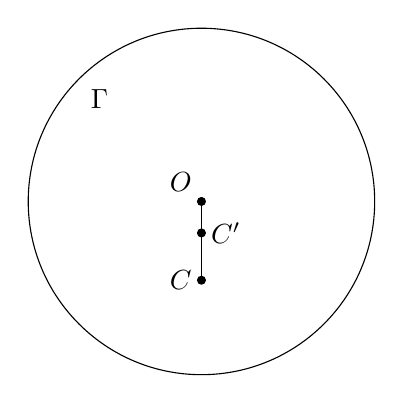
\begin{tikzpicture}[scale=1]
\draw (0,0) circle (2.2cm) node[above left=1.5cm] {$\Gamma$};
\draw (0,0) -- (0,-1);
\draw[fill=black] (0,0) circle (0.05) node[above left] {$O$};
\draw[fill=black] (0,-1) circle (0.05) node[left] {$C$};
\draw[fill=black] (0,-.4) circle (0.05) node[right] {$C'$};
\end{tikzpicture}
\end{center}


%%%%%%%%%%%%%%%%%%%%%%%%%%%%%%%%%%%%%%%%%%%%%%%%%%%%%%%%
\newpage 
\section{The Closure of Fields under Complexification} \label{appendixB}

	Suppose $F$ is a field for which $-1$ is not the square of any number. The complexification of a field $F$ is the process of extending $F$ to a larger set by adding in the an element $i$ such that $i^2 = -1$ and then closing off under addition and multiplication. The resulting field, which we denote $F^\C$ is called the complexification of $F$ or the complexified field $F^\C$. One of the core example of complexification is the complexified reals $\R^\C$. As it turns out, this $\R^\C$ is the complex numbers $\C$. This can also be done to finite fields such as $\Z/3\Z$. Following \cite{complexification}'s derivation, we will prove here that $F^\C$ is a field.

\begin{theorem} 
$\fc$ (as described above) is a field.
\end{theorem}

\begin{proof} Formally, recall that in order for $(F,+,\cdot)$ to be a field, it must satisfy the following axioms:

\begin{enumerate}
	\item $+$ must be associative and commutative.
	\item There exists an additive identity in $F$.
	\item Each $a\in F$ has an additive inverse.
	\item $\cdot$ must be associative and commutative.
	\item $+$ and $\cdot$ satisfy the distributive properties.
	\item There exists an multiplicative identity in $F$.
	\item Each $a\in F$ has an multiplicative inverse.
\end{enumerate}
Previously, all of the algebraic manipulations were carried out over a real ordered field in which all positive numbers have square roots. However, we may also carry out similar calculations over a complexified field. Let $(F,+,\cdot)$ be a field in which $-1$, the additive inverse of $1$, is not the square of any number in $F$. We define $F^\C = F\times F$. Further we define two new binary operations $\oplus$ and $\odot$ such that for all $(a,b)\ttc (c,d)\in F^\C$,
	\[
		(a,b)\oplus(c,d) = (a + c\ttc b + d)
	\]
and
	\[
		(a,b)\odot(c,d) = (ac - bd\ttc ad + bc).
	\]
wherein $+,-,\cdot$ are from $F$. We call $(F^\C,\oplus,\odot)$ the complexification of $F$. From hereon the rest of this section will be dedicated to proving the following theorem.

\begin{theorem}
	Let $(F,+,\cdot)$ be a field in which $-1$ is not a square. Then the complexification $(F^\C,\oplus,\odot)$ as defined above is a field.
\end{theorem}

\noindent First, let's resolve some properties of $\oplus$.\\

\begin{lemma}
	Given a complexification $(F^\C,\oplus,\odot)$, $\oplus$ is associative and commutative.
\end{lemma}

\begin{proof}

First we will show that $\oplus$ is associative. Let $(a,b)\ttc(c,d)\ttc(e,f)\in F^\C$.
\begin{align*}
	((a,b)\oplus(c,d))\oplus(e,f) & = (a + c\ttc b + d) + (e,f)\\
	& = ((a + c) + e\ttc (b + d) + f)\\
	& = (a + (c + e)\ttc b + (d + f)) & \text{(associativity of $+$)}\\
	& = (a,b) \oplus (c + e\ttc d + f)\\
	& = (a,b)\oplus ((c,d) \oplus (e,f))
\end{align*}
Hence $\oplus$ is associative. Now we argue that $\oplus$ is commutative. Let $(a,b)\ttc(c,d)\in F^\C$.
\begin{align*}
	(a,b)\oplus (c,d) & = (a + c\ttc b + d)\\
	& = (c + a\ttc d + b) & \text{(commutativity of $\oplus$)}\\
	& = (c,d)\oplus (a,b)
\end{align*}
Hence $\oplus$ is commutative. 
\end{proof}

Next, we argue that $F^\C$ has an additive identity.\\

\begin{lemma}
	The element $(0,0)\in F^\C$ is an additive identity.
\end{lemma}

\begin{proof}
Let $(a,b)\in F$ be arbitrary. We claim that $(0,0)\in F^\C$ is the additive identity of $F$. Using the fact that $0\in F$ is the additive identity, we obtain
	\[
		(a,b)\oplus (0,0) = (a + 0\ttc b + 0) = (a,b) = (0 + a\ttc, 0 + b) = (0,0) \oplus (a,b).
	\]
Therefore $(0,0)\in F^\C$ is an additive identity.
\end{proof} 

Since $F^\C$ has an additive identity, we may conjecture that $F^\C$ has additive inverses. 

\begin{lemma}
	For all $(x,y)\in F^\C$, there exists $(a,b)\in F^\C$ with 
	\[	
		(x,y)\oplus (a,b) = (0,0) = (a,b)\oplus (x,y).
	\]
	In other words, $F^\C$ has additive inverses.
\end{lemma}

\begin{proof}
Let $(a,b)\in F^\C$ be arbitrary. We claim that $(-a,-b)\in F^\C$ is the additive inverse of $(a,b)$. Note that since $F$ is a field, $-a\ttc -b$ exist and so $(-a,-b)\in F^\C$. Furthermore,
	\[
		(a,b)\oplus (-a,-b) = (a + -a\ttc b + -b) = (0,0) = (-a + a\ttc, -b + b) = (-a,-b) \oplus (a,b).
	\]
	Hence $\oplus$ is closed under inverses.
\end{proof}

Now we've proved that $\oplus$ has the desired properties that addition needs in a field. We therefore set our sights on resolving the properties of $\odot$.\\

\begin{lemma}
	The operation $\odot$ is associative and commutative.
\end{lemma}

\begin{proof}
	Now we argue via a similar line of reasoning that $\odot$ satisfies the properties of field multiplication. First we claim that $\odot$ is associative. Let $(a,b)\ttc(c,d)\ttc(e,f)\in F^\C$ be arbitrary. Using distributivity in $F$ and associativity and commutativity of $+$ and $\cdot$, we obtain
\begin{align*}
		((a,b)\odot(c,d))\odot(e,f) & = (ac - bd\ttc ad + bc)\odot (e,f)\\
		& = ((ac - bd)e - (ad + bc)f\ttc (ac - bd)f + (ad + bc)e)\\
		& = (ace - bde - adf - bcf\ttc acf - bdf + ade + bce)\\
		& = (a(ce - df) - b(de + cf)\ttc b(ce - df) + a(de + cf))\\
		& = (a,b)\odot (ce - df\ttc de + cf)\\
		& = (a,b)\odot ((c,d)\odot (e,f))
\end{align*}
Hence $\odot$ is associative. Now we show that $\odot$ is commutative. Let $(a,b)\ttc(c,d)\in F^\C$ be arbitrary. Then
	\begin{align*}
		(a,b)\odot (c,d) & = (ac - bd\ttc ad + bc)\\
		& = (ca - db\ttc da + cb) & \text{(commutativity of $\cdot$)}\\
		& = (c,d)\odot (a,b)
	\end{align*}
	Therefore $\odot$ is commutative.
\end{proof}

With these properties in mind, we now show that $F^\C$'s operations obey the distributive property.\\

\begin{lemma}
	The complexification $(F^\C,\oplus,\odot)$ obeys the distributive property.
\end{lemma}

\begin{proof}
Next we show that $F^\C$ has the distributive property. Let $(a,b)\ttc(c,d)\ttc(e,f)\in F^\C$ be arbitrary. Since $\odot$ is commutative, it suffices to argue that
	\[
		(a,b)\odot((c,d)\oplus(e,f)) = (a,b)\odot(c,d)\oplus(a,b)\odot(e,f).
	\]
	Following previous arguments, we find that
	\begin{align*}
		(a,b)\odot((c,d)\oplus(e,f)) & = (a,b)\odot(c + e\ttc d + f)\\
		& = (a(c + e) - b(d + f)\ttc a(d + f) + b(c + e))\\
		& = (ac + ae - bd - bf\ttc ad + af + bc + be) & \intertext{(distributivity in $F^\C$)}
		& = ((ac - bd) + (ae - bf)\ttc (ad + bc) + (af + be)) & \intertext{(commutativity and associativity of $+$)}
		& = (ac - bd\ttc ad + bc)\oplus (ae - bf\ttc af + be)\\
		& = (a,b)\odot (c,d)\oplus (a,b)\odot(e,f)
	\end{align*}
	Hence $F^\C$ has the distributive property. 
\end{proof}	

Since $F^\C$ satisfies the distributive property, we only have two properties left to demonstrate: multiplicative identities and multiplicative inverses. \\

\begin{lemma}
	The element $(1,0)\in F^\C$ is a multiplicative identity.
\end{lemma}

\begin{proof}
We claim that $(1,0)$ is the multiplicative identity of $F^\C$. Let $(a,b)\in F^\C$ be arbitrary. Note that since $F$ is a field, $1\in F$ is the multiplicative identity. Then
	\[
		(a,b)\odot(1,0) = (a\cdot 1 - b\cdot 0\ttc a\cdot 0 + b\cdot 1) = (a,b) = (1\cdot a - 0\cdot b\ttc 0\cdot a + 1\cdot b) = (1,0)\cdot (a,b).
	\]
	Hence $F^\C$ has a multiplicative identity.
\end{proof}

Since $F^\C$ has a multiplicative identity, we may conjecture that $F^\C$ has multiplicative inverses. \\
 
\begin{lemma}
	For all $(x,y)\in F^\C\backslash\{(0,0)\}$, there exists $(a,b)\in F^\C\backslash\{(0,0)\}$ with 
	\[	
		(x,y)\odot (a,b) = (1,0) = (a,b)\odot (x,y).
	\]
	In other words, $F^\C$ has multiplicative inverses.	
\end{lemma} 

\begin{proof}
Suppose $(a,b)\in F^\C\backslash\{(0,0)\}$. We hope to find $(x,y)\in F^\C$ with the property $(a,b)\odot(x,y) = (1,0)$. Since $\odot$ is commutative, this result holds for $(x,y)\odot(a,b)$ as well. Performing the multiplication, we find that
	\[
		(a,b)\odot(x,y) = (ax - by\ttc ay + bx) = (1,0)
	\]
	and so we obtain the equations
	\begin{align*}
		ax - by & = 1\\
		ay + bx & = 0
	\end{align*}
	Now we need to solve for $x$ and $y$. Multiply the upper equation by $a$ and the lower equation by $b$ to obtain
	\begin{align*}
		a^2x - aby & = a\\
		aby - b^2x & = 0
	\end{align*}
	Adding the two equations together, we find that
	\[
		x = \frac{a}{a^2 + b^2}.
	\]
	Via a similar process of multiplying the first equation by $b$ and the second equation by $a$ and adding the results, we also obtain
	\[
		y = \frac{-b}{a^2 + b^2}.
	\]
	Now we hope that there is no $(a,b)\in F^\C\backslash\{(0,0)\}$ with $a^2 + b^2 = 0$. Suppose such values do exist however. Since $(a,b)\neq (0,0)$, suppose $a\neq 0$. Then we conclude that
	\begin{align*}
		a^2 + b^2 = 0 & \text{ which implies } b^2 = -a^2\\
		& \text{ which implies } \frac{b^2}{a^2} = -1\\
		& \text{ which implies } \left(\frac{b}{a}\right)^2 = -1.
	\end{align*}
 	In other words, $-1$ is the square of $\frac{b}{a}\in F$, a contradiction since we assumed that no element in $F$ had $-1$ as its square. A similar argument can be made for when $b \neq 0$ using the fraction $\frac{a}{b}$. Hence $a^2 + b^2 \neq 0$ for any $(a,b)\in F^\C\backslash\{(0,0)\}$. Therefore $F^\C$ has multiplicative inverses.
\end{proof} 	
 	
Combining these seven lemmas, we conclude that $(F^\C,\oplus,\odot)$ is a field as desired. Hence the theorem is true and so the complexification of a field is a field. 

\end{proof}



%%%%%%%%%%%%%%%%%%%%%%%%%%%%%%%%%%%%%%%%%%%%%%%%%%%%%%%%
\newpage 
\section{Encoding LFTs as Matrices} \label{appendixC}

\noindent Define the set
	\[
		A = \left\lbrace z\mapsto \frac{az + b}{cz + d}\colon z\in\C\ttc a,b,c,d\in F\text{ with } ad - bc \neq 0\right\rbrace
	\]
of linear fractional transformations under function composition and let $GL_2(F)$ denote the group of invertible $2\times 2$ matrices with entries in $F$. Also define the subset
	\[
		F^* = \left\lbrace\lftmat{\lambda}{0}{0}{\lambda}\colon \lambda\in F\text{ with } \lambda\neq 0 \right\rbrace.
	\]
	We argue that $F^*$ is a normal subgroup of $GL_2(F)$.
\begin{lemma}\label{thm:PGL2F}
	The subset $F^*$ defined above forms a normal subgroup of $GL_2(F)$.
\end{lemma}
\begin{proof}
	Let $F^*$ be defined as above. We first argue that $F^*$ is a subgroup of $GL_2(F)$. Let $A,B\in F^*$ be arbitrary. Then
	\[
		AB = \lftmat{\lambda_A}{0}{0}{\lambda_A}\lftmat{\lambda_B}{0}{0}{\lambda_B} = \lftmat{\lambda_A\lambda_B}{0}{0}{\lambda_A\lambda_B}
	\]
	and since $\lambda_A\lambda_B\in F$ and $F$ has no zero divisors, we conclude that $AB\in F^*$. It's worth noting that the matrices in $F^*$ commute with one another since $\lambda_A\lambda_B = \lambda_B\lambda_A$. From here, notice that the identity element of $F^*$ remains the identity matrix as
	\[
		AI = \lftmat{\lambda_A}{0}{0}{\lambda_A}\lftmat{1}{0}{0}{1} = A
	\]
	and $IA = A$ by commutativity. In a similar vein, if $A\in F^*$ has entry $\lambda_A$, then $B\in F^*$ with $\lambda_B = \frac{1}{\lambda_A}$ is the inverse of $A\in F^*$, following from the assumption that $\lambda_A \neq 0$. Hence $F^*$ forms a subgroup of $GL_2(F)$. Now we show that $F^*$ is normal. Let $A\in GL_2(F)$ and choose some $B\in F^*$. We argue that $AB = CA$ for some $C\in F^*$. Observe that
	\[
		AB = \stanlftmat\lftmat{\lambda_B}{0}{0}{\lambda_B} = \lftmat{a\lambda_B}{b\lambda_B}{c\lambda_B}{d\lambda_B} = \lftmat{\lambda_B a}{\lambda_B b}{\lambda_B c}{\lambda_B d} = \lftmat{\lambda_B}{0}{0}{\lambda_B}\stanlftmat = BA.
	\]
	Therefore $F^*$ is normal as desired.
\end{proof}

The quotient group formed here is known as $PGL(2,F)$, the projective general linear group of $2\times 2$ matrices with coefficients in $F$.

	To begin discussing a group homomorphisms, we need to know that $A$ under function composition forms a group. 
	
\begin{theorem}
	The set of linear fractional transformations given by $A$ forms a group under function composition.
\end{theorem}

\begin{proof}
	See \cite{shuman_lfts}.
\end{proof}
	
With this in mind, we now define the map $\varphi\colon A\rightarrow PGL(2,F)$ by

	\[
		\varphi\left(z\mapsto \frac{az + b}{cz + d}\right) = \stanlftmat F^*
	\]
	We claim that $\varphi$ is a surjective homomorphism.
\begin{theorem}\label{thm:function_correspondence}
	The map $\varphi\colon A\rightarrow PGL(2,F)$ given above is a surjective homomorphism with $\ker(\varphi)$ given by the set
		\[
			\left\lbrace z\mapsto \frac{az + b}{cz + d}\colon a = d; d \neq 0\text{ and } b = c = 0\right\rbrace.
		\]
\end{theorem}

Before we proceed to prove that this map is a surjective homomorphism, it is questionable as to whether $\varphi$ is well-defined. For example, if $\lambda \neq 0$ with $az + b = ez\lambda + f\lambda$ and $cz + d = gz\lambda + h\lambda$, then the maps
\[
	z\mapsto\frac{az + b}{cz + d}\quad\text{ and }\quad z\mapsto\frac{ez\lambda + f\lambda}{gz\lambda + h\lambda}
\]  
are the same despite having two different representations. Therefore under $\varphi$, they should represent the same element. Of course, this criterion for equal transformations might not be exhaustive. Therefore we have the following lemma.

\begin{lemma}
	The map $\varphi$ is well-defined.
\end{lemma}

\begin{proof}
	First we argue that two maps $f_1(z) = \frac{a_1z + b_1}{c_1z + d_1}$ and $f_2(z) = \frac{a_2 z + b_2}{c_2 z + d_2}$ in $A$ are equal if and only if $s_1 = \lambda s_2$ for some $\lambda\neq 0$ and for all $s\in\{a,b,c,d\}$. Stated another way, all the coefficients of $f_1$ differ by the same nonzero multiple from $f_2$.
	
	Supposing that $f_1 = f_2$, we then have that
	\[
		\frac{a_1z + b_1}{c_1z + d_1} = \frac{a_2 z + b_2}{c_2 z + d_2}.
	\]
	Moreover we have
	\[
		(a_1z + b_1)(c_2z + d_2) = (a_2z + b_2)(c_1z + d_1)
	\]
	or more verbosely 
	\[
		 a_1c_2z^2 + (a_1d_2 + b_1c_2)z + b_1d_2 = a_2c_1z^2 + (a_2d_1 + b_2c_1)z + b_2d_1.
	\]
	Subtracting the right hand side from the left hand side, we then have that
	\begin{equation}
		(a_1c_2 - a_2c_1)z^2 + (a_1d_2 + b_1c_2 - a_2d_1 - b_2c_1)z + (b_1d_2 - b_2d_1) = 0.	
	\end{equation}
	Now if equation (8) is to be equal to zero, linear independence tells us that each coefficient must separately be zero. Therefore we arrive at the system of equations
	\begin{align*}
		a_1c_2 - a_2c_1 & = 0\\
		a_1d_2 + b_1c_2 - a_2d_1 - b_2c_1 & = 0\\
		b_1d_2 - b_2d_1 & = 0
	\end{align*}
	At a first glance, the first equation and third equation tell us that 
	\begin{align}
		\frac{a_1}{a_2} & = \frac{c_1}{c_2}\\
		\frac{b_1}{b_2} & = \frac{d_1}{d_2}.
	\end{align} 
	However, we need to be careful as some of these cofficients might be zero. If any of these of these cofficients are zero, we have the following argument. 
	
	Without loss of generality, suppose	 $a_1 = 0$. Then by the first equation, $a_2c_1 = 0$. Assuming $a_2 = 0$, we now realize the second equation as 
	\[
		b_1c_2 = b_2c_1 \text{ or that } \frac{b_1}{b_2} = \frac{c_1}{c_2}.
	\]
	Since $\frac{b_1}{b_2} = \frac{d_1}{d_2}$ from the third equation, we've found that all the ratios are equal and so all the coefficients of $f_1$ differ by the same constant multiple from the corresponding coefficients of $f_2$. Now assuming $c_1 = 0$, the second equation becomes
	\[
		b_1c_2 = a_2d_1 \text{ or that } \frac{a_2}{c_2} = \frac{b_1}{d_1}.
	\]
	Reflecting on (10), we conclude that 
	\[
		\frac{b_1}{d_1} = \frac{a_2}{c_2} = \frac{b_2}{d_2}.
	\]
	However this last result mandates $a_2d_2 - b_2c_2 = 0$, which contradictions our assumptions that $f_2\in A$.
	
	Now assume all the cofficients are nonzero. Ideally we would like for 
	\[
		\frac{a_1}{a_2} = \frac{b_1}{b_2} = \frac{c_1}{c_2} = \frac{d_1}{d_2}.
	\] 
	From (9) and (10), we need only show that, for example, $\frac{c_1}{c_2} = \frac{b_1}{b_2}$.	Exploring the middle equation, we find that
	\[
		\frac{c_1}{c_2}a_2d_2 + \frac{d_1}{d_2}b_2c_2 - \frac{b_1}{b_2}a_2d_2 - \frac{a_1}{a_2}b_2c_2 = 0.
	\]
	Exploting (9) and (10), we conclude that
	\[
		\frac{c_1}{c_2}(a_2d_2 - b_2c_2) - \frac{b_1}{b_2}(a_2d_2 - b_2c_2) = 0
	\]
	Since $f_2\in A$, we then conclude that $\frac{b_1}{b_2} = \frac{c_1}{c_2}$ as desired.
	
	Now suppose that $s_1 = \lambda s_2$ for some $\lambda\neq 0$ and for all $s\in\{a,b,c,d\}$. Then following these algebraic manipulations, we conclude that
	\begin{align*}
		\frac{a_1z + b_1}{c_1z + d_1} & = \frac{\lambda a_2z + \lambda b_2}{\lambda c_2z + \lambda d}\\
		& = \frac{\lambda(a_2z + b_2)}{\lambda(c_2z + d_2)}\\
		& = \frac{a_2z + b_2}{c_2z + d_2} & (\lambda \neq 0).
	\end{align*}
	Hence $f_1 = f_2$ if and only if all the coefficients of $f_1$ differ by the same nonzero multiple from $f_2$.
	
	Now that we've characterized the equal functions of $A$, we go forth to prove that $\varphi$ is well-defined. Suppose $f_1,f_2\in A$ are equal. Then
	\[
		\varphi(f_1) = \lftmat{a_1}{b_1}{c_1}{d_1} F^*
	\]
	and 
	\[
		\varphi(f_2) = \lftmat{a_2}{b_2}{c_2}{d_2} F^*
	\]
	Since $f_1 = f_2$, choose $\lambda\neq 0$ for which $s_1 = \lambda s_2$ for all $s\in\{a,b,c,d\}$. In particular, we note that
	\begin{align*}
		\varphi(f_1) & = \lftmat{a_1}{b_1}{c_1}{d_1} F^*\\
		& = \lftmat{\lambda a_2}{\lambda b_2}{\lambda c_2}{\lambda d_2} F^*\\
		& = \lftmat{\lambda}{0}{0}{\lambda}\lftmat{a_2}{b_2}{c_2}{d_2} F^*\\
		& = \lftmat{a_2}{b_2}{c_2}{d_2} F^*.
	\end{align*}
	Therefore $\varphi$ is well-defined.
\end{proof}
	
Now we proceed with the proof of Theorem C.3.	
	
\begin{proof}
	First, we argue that $\varphi$ is a homomorphism. Let $f,g\in A$ be two distinct maps. Notice that
	\begin{align*}
		\varphi(g\circ f) & = \varphi\left(g\left(\frac{a_fz + b_f}{c_fz + d}\right)\right)\\
		& = \varphi\left(\frac{a_g\frac{a_fz + b_f}{c_fz + d_f} + b_g}{c_g\frac{a_fz + b_f}{c_fz + d_f} + d_g}\right)\\
		& = \varphi\left(\frac{a_ga_fz + a_gb_f + b_gc_fz + b_gd_f}{c_ga_fz + c_gb_f + d_gc_fz + d_gd_f}\right) & \text{(simplifying common denominators)}\\
		& = \varphi\left(\frac{(a_ga_f + b_gc_f)z + (a_gb_f + b_gd_f)}{(c_ga_f + d_gc_f)z + (c_gb_f + d_gd_f)}\right) & \text{(grouping terms for $\varphi$)}\\
		& = \lftmat{a_ga_f + b_gc_f}{a_gb_f + b_gd_f}{c_ga_f + d_gc_f}{c_gb_f + d_gd_f} F^*\\
		& = \lftmat{a_g}{b_g}{c_g}{d_g}\lftmat{a_f}{b_f}{c_f}{d_f}F^*\\
		& = \varphi(g)\varphi(f)F^*
	\end{align*}
	Hence $\varphi$ is a homomorphism. Now we argue that $\varphi$ is surjective. Suppose $M F^*\in GL_2(F)/F^*$ is some matrix with entries $a,b,c,d$. Then the linear fractional transformation given by 
	\[
		f(z) = \frac{az + b}{cz + d}
	\]
	is mapped to $M F^*$ by $\varphi$. Hence $\varphi$ is a surjective homomorphism. Now, notice that if a map $f$ is in $\ker(\varphi)$, then 
\end{proof}		
	

\begin{corollary}\label{thm:isomorphism}
	The groups $A/\ker(\varphi)$ and $PGL(2,F)$ are isomorphic.
\end{corollary}
\begin{proof}
	Apply the First Isomorphism Theorem for groups to $A$ using the fact that $\Range(\varphi) = GL_2(F)/F^*$.
\end{proof}

\newpage
\section{Code Simulating LFTs} \label{appendixD}

Below is the code we used to apply point reflections and line reflections to various points in $\C$. 

\lstinputlisting[language=Python]{../python/code.py}

\end{appendices}



%%%%%%%%%%%%%%%%%%%%%%%%%%%%%%%%%%%%%%%%%%%%%%%%%%%%%%%%
\newpage
\bibliographystyle{alpha}
\bibliography{bibliography}

\noindent\todo{[AB][LG] cite the rest of our sources, i guess}

\end{document}
